\documentclass[a4paper, 12pt]{book}

% General Settings
\usepackage[paper = a4paper, margin = 1in]{geometry}
\usepackage[italian]{babel}
\usepackage[utf8]{inputenc}
\usepackage[T1]{fontenc}
\usepackage{hyperref}
\usepackage{graphicx}
\usepackage[small]{caption}
\usepackage{subfig}
\usepackage[usenames,dvipsnames]{xcolor}
\usepackage{graphicx,color,listings}
\usepackage{float}
\usepackage{booktabs}
\usepackage{hologo}
\usepackage{colortbl}

% Math and physic packages
\usepackage{amsmath,amssymb,amsthm}
\usepackage{mathrsfs}
\usepackage{mathdots}
\usepackage{mathtools}
\numberwithin{equation}{section}
\numberwithin{figure}{chapter}

% Quantum and classical circuits packages
\usepackage[braket, qm]{qcircuit}
\usepackage{circuitikz}
\usepackage{physics}

% New or renewed commands
\newcommand{\lecture}[2]{{\scshape{Lezione #1 - #2}} \par}
\newtheorem{definition}{Definizione}[chapter]
\newtheorem{theorem}{Teorema}[chapter]
\newtheorem{esempio}{Esempio}[chapter]
\renewcommand{\thefootnote}{\roman{footnote}}
\newtheorem*{prf}{Dimostrazione}

% Documents
\begin{document}
    \begin{titlepage}
        \begin{center}
            \vspace*{5cm}
            {\scshape\LARGE Università degli Studi di Milano Bicocca \par}
            \vspace{1.0cm}
            \line(1,0){425} \\
            {\huge\bfseries Teoria della materia condensata I \par}
            \line(1,0){425} \\
 	        \vspace{0.5cm}
            {\Large Raccolta di appunti, dispense e libri \par}
            \vspace{1.0cm}
            {Anno accademico 2021/2022 \par}
            \vspace{0.5cm}
            {\bfseries Marco Gobbo \par}
            \vspace{0.5cm}
            {\url{https://github.com/marcogobbo/tecnologie-quantistiche} \par}
            \vspace*{\fill}
            {\large \today \par}
        \end{center}
    \end{titlepage}
    \tableofcontents
    %%%%%%%%%%%%%
% LECTURE 1 %
%%%%%%%%%%%%%

\chapter{Meccanica quantistica}

\lecture{1}{07/10/2021}
\section{Stati e qubit}
Prima di addentrarci nello studio delle tecnologie quantistiche, risulta opportuno fare alcuni richiami di meccanica quantistica implementando alcuni concetti che ci saranno poi utili in futuro. In particolare iniziamo velocemente ricordando il primo postulato della meccanica quantistica
\begin{itemize}
    \item \textbf{I Postulato} (\textbf{Stato}): Che cos'è uno stato? Utilizziamo la notazione di Dirac per rappresentare un vettore $\ket{\psi}$ di uno spazio di Hilbert $\mathcal{H}$ (molto spesso uno spazio vettoriale finito dimensionale) e diremo che $\ket{\psi} \in \mathcal{H}$. Uno stato è un \textbf{raggio} tale che $\norm{\ket{\psi}} = 1$ (per la conservazione della probabilità) e $\ket{\psi} \cong e^{i \alpha} \ket{\psi}$ \footnote{La notazione $\cong$ significa "equivalente a".} con $\alpha \in \mathbb{R}$. Dato che la fase globale è irrilevante, quando due stati differiscono per una fase hanno il medesimo effetto fisico. 
\end{itemize}
Procediamo ora con il definire cosa sia un qubit
\begin{definizione}[\textbf{Qubit}]
    Un qubit è un qualsiasi sistema a due livelli. Ogni sistema quantomeccanico può essere un qubit, ad esempio si può creare utilizzando le due differenti polarizzazioni del fotone, utilizzando l’allineamento dello spin di un nucleo immerso in un campo magnetico uniforme, utilizzando la tecnica della trappola ionica, sistemi superconduttivi, \dots
\end{definizione}
\noindent Davide di Vincenzo, nel 2000, ha indicato cinque criteri necessari per la scelta di un sistema fisico adatto per la computazione quantistica:
\begin{enumerate}
    \item Un sistema fisico scalabile con qubit ben caratterizzati;
    \item La capacità di inizializzare lo stato dei qubit a un semplice stato fiduciale;
    \item Tempi di decoerenza lunghi e rilevanti;
    \item Un insieme "universale" di porte quantistiche;
    \item Una capacità di misurazione specifica per qubit.
\end{enumerate}
La meccanica quantistica si occupa di descrivere il comportamento del nostro sistema a due livelli mediante una hamiltoniana. Per fare ciò lavoriamo in spazi di Hilbert bidimensionali $\mathcal{H}=\mathbb{C}^2$, quindi le hamiltoniane di questi sistemi sono degli operatori definiti su $\mathbb{C}^2 \rightarrow \mathbb{C}^2$. Gli stati in cui si trova il nostro sistema sono descritti da funzioni d'onda generiche $\psi \in \mathbb{C}^2$, in particolar modo possono essere decomposte sulla base computazionale $\{\ket 0, \ket 1\}$. Avremo quindi che 
\begin{equation*}
    \begin{array}{l}
        \hat H \ket 0 = E_0 \ket 0 \\
        \hat H \ket 1 = E_1 \ket 1 \, ,
    \end{array}
\end{equation*}
dove
\begin{equation*}
    \begin{array}{l}
        \ip{0}{0}=\ip{1}{1}=1 \\
        \ip{0}{1}=\ip{1}{0}=0 \, .
    \end{array}
\end{equation*}
Per cui ogni stato generico $\ket \psi$ può essere scritto come combinazione lineare di $\{\ket 0, \ket 1\}$
\begin{equation*}
    \ket \psi = a \ket 0 + b \ket 1 \, ,
\end{equation*}
con $a,b \in \mathbb{C}$ e soddisfacenti la condizione di conservazione di probabilità
\begin{equation*}
    \abs{a}^2+\abs{b}^2=1 \, .
\end{equation*}
Osserviamo che, per come è definito, $\ket \psi$ è uno \textbf{stato puro}, ci dà la massima conoscenza che possiamo ottenere da questo sistema. Infatti abbiamo una probabilità pari a $\abs{a}^2$ di ottenere $\ket 0$ e una probabilità pari a $\abs{b}^2$ di ottenere $\ket 1$. Dobbiamo misurare un numero infinito di volte per poter ottenere queste distribuzioni di probabilità, tuttavia non possiamo eseguire una misura successiva per estrarre ulteriori informazioni sul nostro stato $\ket \psi$ poiché quest'ultimo sarà collassato in $\ket 0$ oppure $\ket 1$. Per determinare univocamente $\alpha$ e $\beta$ si necessiterebbe un'infinità di esperimenti su un'infinità di stati tutti preparati nel medesimo stato $\ket \psi$. La massima conoscenza che possiamo estrarre non è molta, questo fatto è stato oggetto di discussione per molti anni. In particolar modo ci si è chiesti se la teoria meccanica quantistica fosse una teoria completa o meno\footnote{Einstein, A., Podolsky, B., \& Rosen, N. (1935). Can Quantum-Mechanical Description of Physical Reality Be Considered Complete?. Phys. Rev., 47, 777–780.}.\\
Come abbiamo già accennato, $a$ e $b$ sono coefficienti complessi, attraverso la notazione esponenziale possiamo scriverli come
\begin{equation*}
    a=\abs{a}e^{i\theta_0} \qquad b=\abs{b}e^{i\theta_1}\, ,
\end{equation*}
in questo modo
\begin{equation*}
    \begin{aligned}
        \ket \psi &= \abs{a}e^{i\theta_0}\ket 0 + \abs{b}e^{i\theta_1}\ket 1 \\
                  &= \underbrace{e^{i\theta_0}}_{\mathclap{\text{Fase globale}}}\Big(\abs{a}\ket 0 + \abs{b}\underbrace{e^{i\left(\theta_1-\theta_0\right)}}_{\mathclap{\text{Fase relativa}}}\ket 1\Big) \, .
    \end{aligned}
\end{equation*}
Quando misuriamo uno stato, la \textit{fase globale} risulta essere irrilevante, ciò che conta è la \textit{fase relativa} perché può dar luogo a fenomeni come l'interferenza.
\begin{esempio}[Fase relativa]
    Consideriamo gli stati $\ket 0 e \ket 1$, per scrivere i seguenti stati
    \begin{equation*}
        \ket{\psi_1}=\frac{\ket 0 + \ket 1}{\sqrt 2}\, \qquad \ket{\psi_2}=\frac{\ket 0 - \ket 1}{\sqrt 2} 
    \end{equation*}
    In questo caso il segno meno proviene dalla fase relativa. $\ket{\psi_1}$ e $\ket{\psi_2}$ forniscono lo stesso risultato per una misura di energia (lo si può verificare calcolando $\mel{\psi_i}{\hat H}{\psi_i}$), tuttavia riusciamo a distinguerli se facciamo una misura diversa. Ad esempio possiamo considerare la matrice di Pauli
    \begin{equation*}
        \sigma_x = \begin{pmatrix}
                    0 & 1 \\
                    1 & 0
                   \end{pmatrix}\, ,
    \end{equation*}
    $\ket{\psi_1}$ e $\ket{\psi_2}$ sono autostati di $\sigma_x$ con autovalori, rispettivamente, $1$ e $-1$.
\end{esempio}
\noindent Uno dei problemi principali nell'aver a che fare con sistemi quantistici è trovare l'evoluto temporale di un certo stato, perché abbiamo delle hamiltoniane che descrivono ad esempio il rumore degli strumenti, la temperatura dell'ambiente, \dots L'equazione di Schrödinger si comporta bene nel descrivere l'evoluzione di \textbf{sistemi chiusi}, ma un qubit è, in generale, un \textbf{sistema aperto} che si lega a sistemi esterni e quindi la conoscenza sul suo stato tende a diminuire, finché non perdiamo completamente l'informazione che possedeva all'inizio. Questo fatto è legato al \textbf{tempo di coerenza}. Ci sono vari modi per tenere conto di queste interazioni così da poter descrivere al meglio il nostro sistema a due livelli.\\
Supponiamo di avere un sistema chiuso che evolve secondo l'equazione di Schrödinger
\begin{equation*}
    \hat H \ket{\psi(t)}=i\hbar \partialderivative{t}\ket{\psi(t)}\, ,
\end{equation*}
dove $\ket{\psi(t)}=\hat U(t)\ket{\psi(0)}$. $\hat U$ in questo caso è un operatore unitario che può essere espresso, se l'hamiltoniana è costante nel tempo, come
\begin{equation*}
    \hat U(t)=e^{-\frac{i}{\hbar}\hat H t}\, .
\end{equation*}
Pertanto, considerando gli autostati dell'hamiltoniana 
\begin{equation*}
    \hat H \ket{i}=E_i\ket{i}\, ,
\end{equation*}
e riscrivendo il nostro stato iniziale in termini di autostati dell'hamiltoniana
\begin{equation*}
    \ket{\psi(0)}=\sum_i a_i\ket i\, ,
\end{equation*}
possiamo valutare il nostro stato al tempo generico $t$ come
\begin{equation*}
    \ket{\psi(t)}=\sum_i a_ie^{-\frac i \hbar \hat H t}\ket i=\sum_i a_i e^{-\frac i \hbar E_i t}\ket i \qquad \text{dove} \quad a_i(t)=a_i(0)e^{-\frac i \hbar E_i t}\, .
\end{equation*}
Da questo caso generale possiamo trattare il nostro sistema a due livelli, in questo caso l'hamiltoniana sarà
\begin{equation*}
    \hat H = \begin{pmatrix}
        E_0 & 0 \\
        0 & E_1
       \end{pmatrix}\, ,
\end{equation*}
applicando l'equazione di Schrödinger sui coefficienti
\begin{equation*}
    i\hbar\derivative{a_0(t)}{t}=E_0a_0(t)\, ,
\end{equation*}
\begin{equation*}
    i\hbar\derivative{a_1(t)}{t}=E_1a_1(t)\, ,
\end{equation*}
troviamo che il nostro stato finale al tempo generico $t$ sarà
\begin{equation*}
    \ket{\psi(t)}=\underbrace{e^{-\frac{i}{\hbar}E_0t}}_{\text{Fase globale}}\Big(a_0(0)\ket 0 +\underbrace{e^{-\frac{i}{\hbar}(E_1-E_0)t}a_1(0)}_{\text{Fase relativa}}\ket 1\Big)\, .
\end{equation*}
Ancora una volta, la fase globale non produce alcun effetto, ciò che notiamo è che l'evoluzione temporale cambia la fase relativa tra gli stati $\ket 0$ e $\ket 1$. Questo spiega perché se abbiamo una interazione che disturba il nostro sistema possiamo avere un cambio nella fase relativa, questo è dato dal fatto che abbiamo una variazione in termini energetici. Questo disturbo è generato da tutto ciò che è esterno al sistema a due livelli. Se perdiamo il controllo su questa fase, perdiamo tutta l'informazione che abbiamo su $\ket{\psi(t)}$, e se questo accade, non abbiamo più uno stato puro. Per questo motivo necessitiamo qualcosa che vada oltre al concetto di funzione d'onda generica $\psi$.

\section{Matrice densità}
Vogliamo realizzare uno stato puro $\ket \psi$ che sia una combinazione pura di stati $\ket 0$ e $\ket 1$:
\begin{equation*}
    \ket \psi = a\ket 0 + b \ket 1\, ,
\end{equation*}
nella realtà quando cerchiamo di realizzare questo stato, abbiamo un'indeterminazione classica rappresentata da una distribuzione di probabilità di ottenere lo stato esatto oppure uno stato simile. Supponiamo di avere un insieme di stati che indichiamo con $\{p_i, \ket{\psi_i}\}$, dove $p_i$ è la probabilità classica di ottenere un generico stato. Questi stati $\ket{\psi_i}$ sono tutti stati puri, ma non sappiamo quale sia quello giusto e la sua conoscenza è persa. Tutte queste informazioni sono contenute nella \textbf{matrice densità} che rappresenta una distribuzione classica di probabilità.\\
Dal punto di vista della teoria della meccanica quantistica, esiste un altro modo per introdurre la teoria anziché sfruttare gli stati $\psi$. Quello che si fa è sfruttare la matrice densità che è un operatore che agisce nel seguente modo
\begin{equation*}
    \hat \rho \ket{\psi_i}=p_i\ket{\psi_i}\, ,
\end{equation*}
dove $p_i$ rappresenta la probabilità di ottenere lo stato i-esimo. La matrice densità è ora una miscela di stati puri
\begin{equation*}
    \hat \rho = \sum_i p_i \op{\psi_i}{\psi_i}
\end{equation*}
e descrive la mancanza di conoscenza sui sistemi quantistici che avevamo precedentemente. Se utilizzassimo lo stesso operatore $\hat U$ per descrivere l'evoluto temporale di $\ket{\psi_i} \overset{t}{\longrightarrow} \hat U\ket{\psi_i}$, come possiamo applicarlo a $\hat \rho$?
\begin{equation*}
    \hat \rho = \sum_i p_i \op{\psi_i}{\psi_i} \longrightarrow \sum_i p_i \hat U\op{\psi_i}{\psi_i}\hat U^\dagger \,
\end{equation*}
\begin{equation*}
    \hat U \hat \rho \hat U^\dagger = \hat \rho ' \, .
\end{equation*}
Vediamo se le distribuzioni di probabilità classiche, nel caso di stati ortonormali, vengono conservate:
\begin{proof}\mbox{}\\*
    \noindent A $t=0$ :
    \begin{equation*}
          \hat \rho \ket{\psi_i (0)} = p_i \ket{\psi_i (0)} \\
    \end{equation*}
    A $t>0$ :
    \begin{equation*}
        \begin{aligned}
            \hat \rho' \ket{\psi_i (t)} &= \hat U \hat \rho \hat U^\dagger \hat U \ket{\psi_i (0)} \\      
                                        &=\hat U \hat \rho \ket{\psi_i (0)} \\
                                        &=\hat U p_i \ket{\psi_i (0)} \\
                                        &=p_i U \ket{\psi_i (0)} \\
                                        &=p_i\ket{\psi_i (t)}
        \end{aligned}
    \end{equation*}

    \noindent La probabilità $p_i$ non è cambiata nel tempo, ma lo stato sì perché ora è $\ket{\psi_i (t)}$ che non è uguale a $\ket{\psi_i (0)}$.
\end{proof}
    %%%%%%%%%%%%%
% LECTURE 2 %
%%%%%%%%%%%%%
\newpage
\noindent \lecture{2}{08/10/2021}

\section{Osservabili}\label{sec:osservabili}

\begin{itemize}
    \item \textbf{II Postulato} (\textbf{Osservabili}): Che cosa si può misurare in QM? Vengono misurate le \textbf{osservabili}, ossia \textbf{operatori autoaggiunti} (o \textbf{hermitiani}) $\hat{A}$ tali che
    \begin{equation*}
        \hat{A}: \mathcal{H}\rightarrow \mathcal{H} \, \text{ con } \, \hat{A}^\dagger = \hat{A} \, ,
    \end{equation*}
    dove più precisamente $\hat{A}^\dagger \equiv (\hat{A}^t)^\ast$. Dal punto di vista degli elementi di matrice, calcolare l'aggiunto di $A_{ij}$ significa $A^\dagger_{ij} = A^\ast_{ji}$. Dunque le matrici autoaggiunte (hermitiane) sono tali che $A^\dagger \equiv (A^t)^\ast = A$.  
\end{itemize}

\noindent In base a ciò che abbiamo visto sulla notazione braket  ($\bra{\phi} = \ket{\phi}^\dagger$) abbiamo necessariamente che

\begin{equation*}
    \ket{\psi} = B \ket{\phi} \, , \quad \Rightarrow \quad  \bra{\psi} = \bra{\phi} B^\dagger \, .
\end{equation*}

\noindent Focalizzando la nostra attenzione sugli operatori autoaggiunti, richiamiamo un importante teorema di algebra lineare:
\begin{teorema}[\textbf{Teorema Spettrale}]
    Sia $\hat{A}$ un operatore autoaggiunto su uno spazio di Hilbert $\mathcal{H}$. Allora esiste una base ortonormale di $\mathcal{H}$ composta da autovettori di $\hat{A}$, ossia $\exists$ $\lbrace \ket{n} \rbrace \in \mathcal{H}$ tale che $\hat{A} \ket{n} = a_n \ket{n}$ dove gli autovalori $a_n \in \mathbb{R}$.
\end{teorema}

\noindent Si noti dal teorema che $\braket{n}{m} = \delta_{nm}$ dove $n,m = 1, \ldots, N$ con $N \equiv \dim \mathcal{H}$. Trattandosi di una base, qualsiasi vettore dello spazio di Hilbert può essere scritto come combinazione lineare di tali vettori: 

\begin{equation*}
    \ket{\psi} = \sum_{n=1}^N \alpha_n \ket n \, , \, \text{ dove } \, \alpha_n \equiv \braket{n}{\psi} \in \mathbb{C} \, .
\end{equation*}

\noindent Ritornando al nostro caso del sistema a due livelli, lo spazio di Hilbert in esame è $\mathbb{C}^2$, dove consideriamo la \textbf{base canonica} (o \textbf{base computazionale}) data dagli stati $\ket 0$ e $\ket 1$ (si vedano le definizioni in \eqref{computational_basis}). In questo spazio vettoriale gli operatori sono rappresentati da matrici $2 \times 2$. La più generale matrice $2 \times 2$ hermitiana contenente 4 parametri reali è

\begin{equation*}
    A = 
    \begin{pmatrix}
        a+b & c-id \\ 
        c+id & a-b
    \end{pmatrix} \, ,
\end{equation*}

\noindent dove $a, b, c, d \in \mathbb{R}$. Si noti che sulla diagonale le entrate sono puramente reali. Così come abbiamo decomposto uno stato generico $\ket{\psi}$ mediante combinazione lineare di autovettori $\ket{n}$, possiamo decomporre il generico operatore hermitiano di $\mathbb{C}^2$ come 

\begin{equation}\label{generical_matrix_C2}
    A = a \mathbb{I} + c \sigma_1 + d \sigma_2 + b \sigma_3 \, ,
\end{equation}

\noindent dove $\mathbb{I}$ è la matrice \textbf{identità} e $\sigma_1, \sigma_2, \sigma_3$ sono le \textbf{matrici Pauli}:

\begin{equation}\label{Pauli_matrices}
    \sigma_1=
    \begin{pmatrix}
        0 & 1 \\
        1 & 0
    \end{pmatrix} \, , \ \ \ \ \
    \sigma_2=
    \begin{pmatrix}
        0 & -i \\
        i & 0
    \end{pmatrix} \, , \ \ \ \ \
    \sigma_3=
    \begin{pmatrix}
        1 & 0 \\
        0 & -1
    \end{pmatrix} \, . \ \ \ \ \
\end{equation}

\noindent Si ricordi che le matrici di Pauli sono i generatori del momento angolare in QM e sono infatti utilizzate per descrivere l'operatore di spin $\hat{\vec{S}} = \frac{\hbar}{2} \hat{\vec{\sigma}}$. I relativi autovalori e autovettori sono mostrati nella Tabella \ref{tab:Pauli_eig}.

\begin{table}[!ht]
	\centering
    \begin{tabular}{ccc}
        \toprule
        \textbf{Matrice di Pauli} & \textbf{Autovettori} & \textbf{Autovalori}  \\
        \midrule
        $\sigma_1$ & $\ket + = \frac{1}{\sqrt 2} \begin{pmatrix} 1 \\ 1 \end{pmatrix}, \qquad \ket - = \frac{1}{\sqrt 2} \begin{pmatrix} 1 \\ -1 \end{pmatrix} $ & $\lbrace 1, -1 \rbrace$ \\
        $\sigma_2$ & $\ket i = \frac{1}{\sqrt 2} \begin{pmatrix} 1 \\ i \end{pmatrix}, \qquad \ket{-i} = \frac{1}{\sqrt 2} \begin{pmatrix} 1 \\ -i \end{pmatrix} $ & $\lbrace 1, -1 \rbrace$ \\
        $\sigma_3$ & $\ket 0 = \begin{pmatrix} 1 \\ 0 \end{pmatrix}, \qquad \ket 1 = \begin{pmatrix} 0 \\ 1 \end{pmatrix} $ & $\lbrace 1,-1 \rbrace$ \\
        \bottomrule
    \end{tabular}\\
    \caption{Autovettori e autovalori delle matrici di Pauli.}
    \label{tab:Pauli_eig}
\end{table}

\noindent Dato che in futuro ci tornerà utile, osserviamo che gli autovettori di $\sigma_1$ e $\sigma_2$ possono essere espressi mediante base computazionale come

\begin{equation}\label{basi_di_sigma_12}
    \ket + = \frac{\ket 0 + \ket 1}{\sqrt 2} \, , \quad \ket - = \frac{\ket 0 - \ket 1}{\sqrt 2} \, , \quad \ket i = \frac{\ket 0 + i \ket 1}{\sqrt 2} \, , \quad \ket{-i} = \frac{\ket 0 - i \ket 1}{\sqrt 2} \, ,
\end{equation}

\noindent Utilizzando la rappresentazione dei qubit tramite sfera di Bloch, questi autovettori sono mostrati in Figura \ref{fig:BlochSphere2}. 

\begin{figure}[!ht]
    \centering
    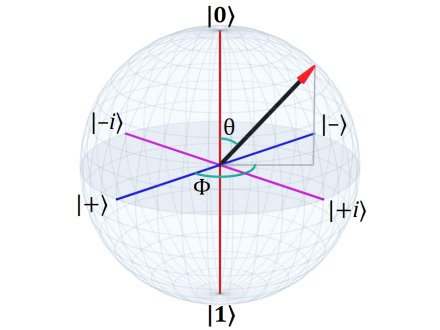
\includegraphics[scale=0.6]{images/bloch-hdr-440.png}
    \caption{Rappresentazione degli autovettori delle matrici di Pauli sulla sfera di Bloch. Il punto indicato dalla freccia rossa indica un generico qubit.}
    \label{fig:BlochSphere2}
\end{figure}

\noindent Come detto in precedenza, le 3 matrici di Pauli parametrizzano lo spin e i 3 assi della sfera di Bloch possono essere associati allo spin. Considerando lo stato generico $\ket{\psi}$ della \eqref{generic qubit}, possiamo definire lo spin lungo una direzione generica $\vec{\sigma} \cdot \vec{n}$ dove $\vec n = (\cos\phi\sin\theta, \sin\phi\sin\theta, \cos\theta)$:

\begin{equation*}
    \vec{\sigma} \cdot \vec n = \cos\phi\sin\theta \, \sigma_1 + \sin \phi \sin \theta \, \sigma_2 + \cos \theta \, \sigma_3 \, ;
\end{equation*}
così facendo è un semplice esercizio di QM dimostrare che $\ket{\psi}$ è autostato di $\vec{\sigma} \cdot \vec n$ con autovalore 1, ossia $\vec{\sigma} \cdot \vec n \ket{\psi} = \ket{\psi}$. Questo significa che dato uno stato sulla sfera di Bloch, allora esso è anche autostato di spin nella direzione individuata da tale qubit: infatti l'idea fisica alla base della sfera di Bloch è che la direzione arbitraria scelta non è altro che la direzione della quantizzazione dello spin. 

\section{Misurazioni}

\begin{itemize}
    \item \textbf{III Postulato} (\textbf{Regola di Born}):
    \begin{enumerate}
        \item \textbf{Misurazione}: sia $\hat{A}$ un osservabile con autostati $\ket{n}$, ossia $\hat{A} \ket{n} = a_n \ket{n}$. Prendiamo per semplicità $a_n \neq a_m \ \forall \, n \neq m$ (osservabile con autovalori distinti). Consideriamo uno stato generico espanso sugli autostati precedenti: $\ket \psi = \sum_n \alpha_n \ket n$. Allora una misura dell'osservabile $\hat{A}$ produce il valore $a_n$ con probabilità data da $\abs{\alpha_n}^2$ (assumendo lo stato correttamente normalizzato).
        
        \item \textbf{Collasso dello stato}: cosa succede allo stato del sistema dopo la misurazione? Istantaneamente lo stato $\ket \psi$ collassa sull'autostato associato all'autovalore risultante dalla misura. Ad esempio se misurando otteniamo $a_n$ allora $\ket{\psi} \rightarrow \ket{n}$. Effettuando delle misure successive sullo stato si ottiene sempre $\ket{n}$ con probabilità esattamente uguale a 1.  
    \end{enumerate}
\end{itemize}

\begin{esempio}
    Consideriamo per esempio il generico qubit in \eqref{generic qubit} e immaginiamo di voler effettuare delle misurazioni in differenti basi. Supponiamo di voler misurare lo spin lungo $z$ (base $\lbrace \ket{0}, \ket{1} \rbrace$ di $\sigma_3$) e lungo $x$ (base $\lbrace \ket{+}, \ket{-} \rbrace$ di $\sigma_1$). Essendo il qubit già decomposto sulla base computazionale, una misurazione lungo $z$ produrrà
    
    \begin{equation*}
        P(\ket{0}) = \abs{\cos \! \left( \frac{\theta}{2} \right)}^2 \, , \qquad P(\ket{1}) = \abs{\sin \! \left( \frac{\theta}{2} \right)}^2 \, .
    \end{equation*}
    
    \noindent Per capire il risultato della misurazione lungo $x$, invece, dobbiamo espandere $\ket{\psi}$ sulla base $\lbrace \ket{+}, \ket{-} \rbrace$: usando le \eqref{basi_di_sigma_12} per esprimere $\lbrace \ket{0}, \ket{1} \rbrace$ in termini di $\lbrace \ket{+}, \ket{-} \rbrace$ ricaviamo
    
    \begin{equation*}
        P(\ket{+}) = \frac{1}{2} \abs{\cos \! \left( \frac{\theta}{2} \right) + e^{i \phi} \sin \! \left( \frac{\theta}{2} \right)}^2 \, , \qquad P(\ket{-}) = \frac{1}{2} \abs{\cos \! \left( \frac{\theta}{2} \right) - e^{i \phi} \sin \! \left( \frac{\theta}{2} \right)}^2 \, .
    \end{equation*}
    
    \noindent Si noti come in entrambe le situazioni la probabilità risulta correttamente normalizzata: $P(\ket{0}) + P(\ket{1}) = P(\ket{+}) + P(\ket{-}) = 1$. 
\end{esempio}

\begin{esempio}
    Consideriamo lo stato $\ket{+}$ delle \eqref{basi_di_sigma_12}. Qual è l'interpretazione fisica di tale stato? Supponiamo che rappresenti lo spin di una particella: quando lo spin si trova in $\ket{+}$ allora sappiamo con certezza che punta lungo la direzione $x$, ossia $P(\ket{+}) = 1$. Al contrario, per una misurazione lungo $z$ sappiamo che $P(\ket{0}) = 1/2$ e $P(\ket{1}) = 1/2$: abbiamo la certezza del risultato lungo l'asse $x$, ma lungo l'asse $z$ si ha totale incertezza. Questo fenomeno è dovuto alla non commutatività degli operatori di spin nelle 3 direzioni:
    
    \begin{equation*}
        \comm{\hat{S}_i}{\hat{S}_j} = i \hbar \varepsilon_{ijk} \hat{S}_k \, .
    \end{equation*}
    
    \noindent Se consideriamo infatti il sistema preparato in $\ket{+}$ e supponiamo di effettuare una misura lungo $z$ ottenendo $\ket{0}$ allora lo stato collasserà in $\ket{0}$ e, d'ora in avanti, qualsiasi misurazione lungo $z$ produrrà sempre $\ket{0}$ con $P(\ket{0}) = 1$. Nonostante ciò, il fatto che $\hat{S}_z$ non commuti con $\hat{S}_x$ fa sì che una misura successiva lungo $x$ "rigeneri" dell'incertezza: $P(\ket{+}) = 1/2$ e $P(\ket{-}) = 1/2$ (si veda $\ket{0}$ espresso in termini di $\lbrace \ket{+}, \ket{-} \rbrace$ dalle \eqref{basi_di_sigma_12}). 
\end{esempio}

\noindent Discutiamo la generalizzazione del III postulato nel caso in cui alcuni autovalori associati ad autostati differenti siano uguali, cioè siamo in presenza di \textbf{degenerazione}. Per esempio supponiamo il caso $N = \dim \mathcal{H} = 6$: 

\begin{equation*}
    \ket \psi = \alpha_1 \ket 1 + \alpha_2 \ket 2 + \alpha_3 \ket 3 + \alpha_4 \ket 4 + \alpha_5 \ket 5 + \alpha_6 \ket 6 \, , 
\end{equation*}

\noindent dove supponiamo la degenerazione su $a_1 = a_2$ e $a_4 = a_5 = a_6$. Introduciamo gli operatori $\hat{P}_{a_i}$ che considerano solamente la parte di $\ket{\psi}$ corrispondente all'autospazio associato ad $a_i$:

\begin{equation*}
    \ket \psi = \underbrace{\alpha_1 \ket 1 + \alpha_2 \ket 2 }_{\hat P_{a_1} \ket \psi} + \underbrace{\alpha_3 \ket 3}_{\hat P_{a_3} \ket \psi} + \underbrace{\alpha_4 \ket 4 + \alpha_5 \ket 5 + \alpha_6 \ket 6}_{\hat P_{a_4 \ket \psi}} \, ;
\end{equation*}

\noindent tali operatori prendono il nome di \textbf{proiettori} e soddisfano le proprietà seguenti:  
\begin{enumerate}
    \item $\hat P_{a_i}^\dagger = \hat P_{a_i}$;
    \item $\hat P_{a_i}^2 = \hat P_{a_i}$;
    \item $\sum_i \hat P_{a_i} = \mathbb{I}$. 
\end{enumerate}

\noindent I proiettori sono utili per scrivere la \textbf{regola di Born} (III postulato) nel caso generale: dato uno stato $\ket{\psi}$ con degenerazione sugli autovalori $a_i$, la probabilità di ottenere il risultato $a_n$ è

\begin{equation*}
    P(a_n) = \norm{\hat{P}_{a_n} \ket{\psi}}^2 \, ;
\end{equation*}

\noindent dopo la misura, la funzione d'onda collassa nel seguente stato normalizzato:

\begin{equation*}
    \ket{\psi} \rightarrow \frac{\hat{P}_{a_n} \ket{\psi}}{\norm{\hat{P}_{a_n} \ket{\psi}}} \, .
\end{equation*}

\noindent Ad esempio, nel caso dello stato sopra scritto, la probabilità di ottenere $a_1 = a_2$ non è altro che 

\begin{equation*}
    P(a_1) = \norm{\hat{P}_{a_1} \ket{\psi}}^2 = \norm{\alpha_1 \ket{1} + \alpha_2 \ket{2}}^2 = \abs{\alpha_1}^2 + \abs{\alpha_2}^2 \, ,
\end{equation*}

\noindent e lo stato collassa in

\begin{equation*}
    \ket{\psi} \rightarrow \frac{\alpha_1 \ket{1} + \alpha_2 \ket{2}}{\sqrt{\abs{\alpha_1}^2 + \abs{\alpha_2}^2}} \, ;
\end{equation*}

\noindent si noti che si ha ancora incertezza su in quale stato si trovi $\ket{\psi}$, ma con un esperimento successivo \textbf{diverso} siamo in grado di risolvere la degenerazione e ottenere $\ket{1}$ o $\ket{2}$. 

\section{Evoluzione temporale}
Il postulato successivo riguarda l'evoluzione temporale degli stati:

\begin{itemize}
    \item \textbf{IV Postulato} (\textbf{Evoluzione temporale}): L'evoluzione temporale di uno stato generico $\ket{\psi(0)}$ è descritta dall'equazione di Schrödinger:
    
    \begin{equation*}
        i \hbar \dv{t} \ket{\psi(t)} = \hat H \ket{\psi(t)} \, ,
    \end{equation*}
    
    \noindent dove $\hat{H}$ è l'operatore (hermitiano) \textbf{hamiltoniana} del sistema. L'equazione di Schrödinger conserva le probabilità: $\braket{\psi(t)} = \braket{\psi(0)} = 1$. 
\end{itemize}

\noindent Solitamente si risolve questa equazione introducendo l'\textbf{operatore di evoluzione temporale} $\hat{U}(t)$:

\begin{equation*}
    \ket{\psi(t)} = \hat{U}(t) \ket{\psi(0)} \, ;
\end{equation*}

\noindent quando l'hamiltoniana è indipendente dal tempo, $\hat{U}(t)$ diventa semplicemente

\begin{equation*}
    \hat{U} (t) = e^{-\frac{i}{\hbar} \hat H t} \, ;
\end{equation*}

\noindent se invece $\hat H = \hat H(t)$, è necessario distinguere i casi di hamiltoniane commutanti o non commutanti a tempi differenti.\\
\noindent Come detto sopra, l'evoluzione temporale preserva le probabilità e ciò è una diretta conseguenza del fatto che $\hat{U}(t)$ sia \textbf{unitario}: 
\begin{itemize}
    \item $\hat U \hat U^\dagger = \hat U^\dagger U = \mathbb{I} \quad \Rightarrow \quad \hat{U}^\dagger = \hat{U}^{-1}$.
    \item Il prodotto scalare è conservato: $\braket{\hat U\phi}{\hat U\psi} = \braket{\phi}{\hat U^\dagger \hat U\psi} = \braket{\phi}{\psi}$. 
\end{itemize}
\noindent Notiamo che $\hat{U}(t)$ per hamiltoniane indipendenti da $t$ è effettivamente unitario:

\begin{equation*}
    \hat U^\dagger \hat U = \left( e^{-\frac{i}{\hbar} \hat H t} \right)^\dagger e^{-\frac{i}{\hbar} \hat H t} = e^{\frac{i}{\hbar} \hat H t} e^{-\frac{i}{\hbar} \hat H t} = \mathbb{I} \, .
\end{equation*}

\section{Gate}\label{sec:gate}

\begin{definizione}[\textbf{Porte quantistiche}]
    L'analogo quantistico delle porte (o gate) logiche classiche sono le \textbf{porte quantistiche} (o \textbf{gate quantistici}). Un gate quantistico è un operatore unitario che cambia lo stato del sistema.
\end{definizione}

\noindent Notiamo che una delle principali differenze che rendono di difficile implementazione le porte quantistiche risiede nel fatto che non possiamo implementare direttamente le più semplici operazioni classiche come \texttt{AND}, \texttt{OR} o \texttt{XOR}. 

\begin{definizione}[\textbf{Circuito Quantistico}]
    Un \textbf{circuito quantistico} è un modello di computazione quantistica in cui una sequenza ordinata di gate quantistici è applicata ai qubit.
\end{definizione}

\noindent In un circuito classico l'uso dei gate logici è banale. Supponiamo di considerare un bit che si trova in 0 o 1: un gate costituisce l'implementazione di un agente esterno che cambia lo stato del bit. Si pensi ad esempio al gate \texttt{NOT} per il quale $a \rightarrow$ \texttt{NOT} $a$:
\begin{center}
    \begin{circuitikz}
        \draw
        (0,4.5) node[not port] (mynot) {}
        (mynot.in) node[left = .4cm, anchor=east] (a) {$0$}
        (mynot.out) node[right = .4cm,anchor=west] (b) {$1 \, ,$}
        (mynot.in) -- (a)
        (mynot.out) -- (b);
    \end{circuitikz}
    $\qquad$
    \begin{circuitikz}
        \draw
        (0,4.5) node[not port] (mynot) {}
        (mynot.in) node[left = .4cm, anchor=east] (a) {$1$}
        (mynot.out) node[right = .4cm,anchor=west] (b) {$0 \, ,$}
        (mynot.in) -- (a)
        (mynot.out) -- (b);
    \end{circuitikz}
\end{center}

\noindent Nel caso invece di un qubit, i circuiti funzionano diversamente perché le porte agiscono su sistemi a due livelli. Immaginiamo che a causa di un agente esterno il qubit $\ket{\psi}$ subisca un evoluzione temporale $\hat{U}$: rappresentiamo questo fatto mediante il circuito seguente
\begin{center}
    \mbox{
        \Qcircuit @C=2em @R=2em {
            \lstick{\ket{\psi}} & \gate{\hat{U}} & \rstick{\hat{U} \ket{\psi} \, ,} \qw \\
        }
    }
\end{center}

\noindent Si ricordi che $\hat{U}$ è sempre un operatore unitario: ad esempio per un'hamiltoniana indipendente dal tempo si ha semplicemente $\hat{U}(t) = e^{-\frac{i}{\hbar}\hat H t}$. \\
\noindent Consideriamo le matrici di Pauli: sappiamo che sono hermitiane ($\sigma^\dagger_i = \sigma_i$) e che soddisfano la proprietà $\sigma_i^2 = \mathbb{I}$, ma questo significa che sono anche matrici unitarie. Questo fatto ci permette di costruire\footnote{Un tale sistema in natura è abbastanza semplice da implementare poiché, essendo $\hat{H} = \vec{\sigma} \cdot \vec B$ l'accoppiamento tra spin e campo magnetico, è facile costruire una tale evoluzione temporale.} dei gate in cui $\hat{U} = \hat{\sigma}_i$.  Ad esempio è possibile implementare dei gate come $\mathbb{I}$, $\sigma_1 \equiv X$, $\sigma_2 \equiv Y$ e $\sigma_3 \equiv Z$. Ricordando che $\sigma_i \sigma_j = i \varepsilon_{ijk} \sigma_k$ per $i \neq j$, notiamo che $XZ = - i Y$ e inoltre anche la matrice $-iY$ è unitaria. Per tale ragione molto spesso, al posto di considerare i gate $\lbrace \mathbb{I}, X, Y, Z \rbrace$ si sceglie la base $\lbrace \mathbb{I}, X, Z, XZ \rbrace$: questo significa che possiamo implementare i gate seguenti
\begin{center}
    \mbox{
        \Qcircuit @C=2em @R=2em {
            & \gate{X} & \qw \\
        }
    } 
    , \ \ \ \ 
    \mbox{
        \Qcircuit @C=2em @R=2em {
            & \gate{Z} & \qw \\
        }
    }
    , \ \ \ \ 
    \mbox{
        \Qcircuit @C=2em @R=2em {
            & \gate{XZ} & \qw \\
        }
    }
    ,
\end{center}

\noindent Consideriamo l'\texttt{X-gate}: dalle \eqref{Pauli_matrices} è evidente che $X$ rappresenta una sorta di "quantum" \texttt{NOT} perché inverte semplicemente lo stato della base computazionale:
\begin{center}
    \mbox{
        \Qcircuit @C=2em @R=2em {
            \lstick{\ket{0}} & \gate{X} & \rstick{\ket{1} \, ,} \qw \\
        }
    } 
    \\
    \mbox{
        \Qcircuit @C=2em @R=2em {
            \lstick{\ket{1}} & \gate{X} & \rstick{\ket{0} \, ,} \qw \\
        }
    }
\end{center}

\noindent Consideriamo ora lo \texttt{Z-gate}: gli stati della base computazionale sono autovettori con autovalori 1 e $-1$ di $\sigma_3$, quindi questo gate inverte semplicemente il segno
\begin{center}
    \mbox{
        \Qcircuit @C=2em @R=2em {
            \lstick{\ket{0}} & \gate{Z} & \rstick{\ket{0} \, ,} \qw \\
        }
    } 
    \\
    \mbox{
        \Qcircuit @C=2em @R=2em {
            \lstick{\ket{1}} & \gate{Z} & \rstick{-\ket{1} \, ,} \qw \\
        }
    }
\end{center}
L'azione dello \texttt{Z-gate} su un generico qubit risulterà quindi in
\begin{center}
    \mbox{
        \Qcircuit @C=2em @R=2em {
            \lstick{a \ket{0} + b \ket{1}} & \gate{Z} & \rstick{a \ket{0} - b \ket{1} \, ,} \qw \\
        }
    } 
\end{center}
e questo significa che $Z$ aggiunge semplicemente una fase $e^{i \pi} = -1$ allo stato. Ricapitolando: l'\texttt{X-gate} implementa un'interferenza dall'esterno che inverte lo stato (ad esempio cambia segno dello spin lungo $z$) e lo \texttt{Z-gate} implementa l'introduzione di una fase. \\
\noindent Una matrice particolarmente importante per i nostri scopi è 
\begin{equation}\label{Hadamard_matrix}
    H = \frac{1}{\sqrt{2}} 
    \begin{pmatrix}
        1 & 1 \\ 1 & -1 
    \end{pmatrix} \, , 
\end{equation}
chiamata \textbf{matrice di Hadamard}. Notiamo che è unitaria in quanto $H^\dagger H = \mathbb{I}$. Essa può essere implementata nel cosiddetto \texttt{H-gate} o \textbf{gate di Hadamard}: si tratta di un gate particolarmente importante (lo useremo largamente durante tutto il corso) in quanto permette di cambiare base $\lbrace \ket{0}, \ket{1} \rbrace \leftrightarrow \lbrace \ket{+}, \ket{-} \rbrace$ 

\begin{center}
    \mbox{
        \Qcircuit @C=2em @R=2em {
            \lstick{\ket{0}} & \gate{H} & \rstick{\ket{+} \, ,} \qw \\
        }
        \ \ \ \ \ \ \ \ \ \ \ \ \ \ \ \ \ \ \ \ 
        \Qcircuit @C=2em @R=2em {
            \lstick{\ket{+}} & \gate{H} & \rstick{\ket{0}\, ,} \qw \\
        }
    }
    \\
    \mbox{
        \Qcircuit @C=2em @R=2em {
            \lstick{\ket{1}} & \gate{H} & \rstick{\ket{-} \, ,} \qw \\
        } 
        \ \ \ \ \ \ \ \ \ \ \ \ \ \ \ \ \ \ \ \ 
        \Qcircuit @C=2em @R=2em {
            \lstick{\ket{-}} & \gate{H} & \rstick{\ket{1} \, ,} \qw \\
        }
    }
\end{center}

\noindent Possiamo introdurre anche le matrici seguenti (ci serviranno più avanti)

\begin{equation}\label{S_T_matrices}
    S \equiv \sqrt{Z} =
\begin{pmatrix}
    1 & 0 \\ 0 & i
\end{pmatrix} \, , \qquad 
T \equiv \sqrt{S} =
\begin{pmatrix}
    1 & 0 \\ 0 & e^{i \frac{\pi}{4}}
\end{pmatrix} \, ,
\end{equation}

\noindent Le matrici introdotte in precedenza costituiscono gli oggetti base con cui andremo a implementare diversi gate e circuiti durante tutto il corso. Per costruire il gate più generale possiamo esponenziare scrivendo $U = e^{-\frac{i}{\hbar} H t}$ dove $H = a \mathbb{I} + b_i \sigma_i$ e $a, b_i \in \mathbb{R}$ con $i = 1,2,3$. Esiste una particolare classe di operatori che utilizzeremo molto dati da
\begin{equation*}
    R_{\vec{n}}(\lambda) = e^{-i \frac{\lambda}{2} (\vec n \cdot \vec \sigma)} \, ;
\end{equation*}
si tratta di un caso particolare dell'esponenziazione precedente in cui $a = 0$ e i coefficienti $b_i$ sono scelti lungo un particolare versore $\vec n$. Questo operatore unitario implementa una rotazione di angolo $\lambda$ attorno alla direzione individuata da $\vec n$:

\begin{equation}\label{rotation_n_lambda}
    R_{\vec{n}}(\lambda) = e^{-i \frac{\lambda}{2} (\vec n \cdot \vec \sigma)} = \cos \! \left( \frac{\lambda}{2} \right) \mathbb{I} - i \sin \! \left( \frac{\lambda}{2} \right) \vec \sigma \cdot \vec n \, ;
\end{equation}
(si espanda il LHS con la serie di Taylor dell'esponenziale e si usi $(\vec \sigma \cdot \vec n)^2 = \mathbb{I}$ per dimostrare l'uguaglianza con il RHS). È possibile dimostrare, inoltre, che qualsiasi matrice unitaria $2 \times 2$ può essere scritta nella forma seguente
\begin{equation}\label{general_2by2_matrix}
    U = e^{i \alpha}
    \begin{pmatrix}
        e^{-i \frac{\beta}{2}} & 0 \\ 0 & e^{i \frac{\beta}{2}}
    \end{pmatrix}
    \begin{pmatrix}
        \cos \frac{\gamma}{2} & - \sin \frac{\gamma}{2} \\ \sin  \frac{\gamma}{2} & \cos \frac{\gamma}{2}
    \end{pmatrix}
    \begin{pmatrix}
        e^{-i \frac{\delta}{2}} & 0 \\ 0 & e^{i \frac{\delta}{2}}
    \end{pmatrix}
    = e^{i \alpha} R_z(\beta) R_x(\gamma) R_z(\delta) \, ; 
\end{equation}
perciò il più generale operatore unitario presenta 4 parametri reali $\alpha, \beta, \gamma, \delta \in \mathbb{R}$ e può implementare un possibile gate in un computer quantistico. Appare subito evidente come la scelta di 4 possibili parametri reali (quindi continui) consenta di realizzare un numero nettamente maggiore di gate logici quantistici rispetto al caso dei gate logici classici. 
    \vspace{1cm}
\newline
\lecture{3}{14/10/2021}
\vspace{0.5cm}
\noindent Abbiamo visto come sia possibile calcolare il valore di aspettazione di $\expval{A}$ a partire dalle funzioni d'onda. Vogliamo vedere come sia possibile sfruttare la matrice densità per ottenere il medesimo risultato. Cominciamo considerando il generico insieme di stati $\{p_i, \ket{\psi_i}\}$ e la matrice densità corrispondente $\hat \rho=\sum_i p_i\op{\psi_i}{\psi_i}$. Per il singolo stato $\ket{\psi_i}$ avevamo visto che
\begin{equation*}
    \begin{aligned}
        \expval{A}_{\psi_i} &= \sum_k p_k a_k \\
                            &= \sum_k \ip{\psi_i}{a_k}\ip{a_k}{\psi_i}a_k \\
                            &= \bra{\psi_i}\sum_k a_k \ket{a_k}\ip{a_k}{\psi_i} \\
                            &= \expval{A}{\psi_i}
    \end{aligned}
\end{equation*}
Tuttavia, nel caso della matrice densità, abbiamo un insieme di funzioni d'onda, per cui
\begin{equation*}
    \begin{aligned}
        \expval{A} &= \sum_i p_i \expval{\hat A}{\psi_i} \\
                   &= \sum_i p_i \Tr \left(\hat A\op{\psi_i}{\psi_i}\right) \\
                   &= \Tr \left(A\sum_i p_i \op{\psi_i}{\psi_i}\right) \\
                   &= \Tr\left(\hat A\rho\right) \, .
    \end{aligned}
\end{equation*}

\subsection*{Equazione di von-Neumann - Liouville}
Per il \textbf{IV Postulato}, riguardante l'evoluzione temporale, la matrice densità evolve come $\hat U \hat \rho \hat U^\dagger$, ci chiediamo se sia possibile realizzare un'equazione analoga a quella di Schrödinger per la matrice densità. La risposta è affermativa, infatti
\begin{equation*}
    \begin{aligned}
        \derivative{\hat \rho}{t} &= \sum_i p_i\left(\derivative{\ket{\psi_i}}{t}\bra{\psi_i}+\ket{\psi_i}\derivative{\bra{\psi_i}}{t}\right) \\
                                  &= \sum_i \frac{p_i}{i\hbar}\left(\hat H \op{\psi_i}{\psi_i}-\op{\psi_i}{\psi_i}\hat H\right) \\
                                  &= \frac{1}{i\hbar}\comm{\hat H}{\hat \rho}
    \end{aligned}
\end{equation*}

\noindent Consideriamo ora un paio di esempi per assodare i concetti finora trattati
\begin{esempio}
    Consideriamo un qubit nella base computazionale $\{\ket 0, \ket 1\}$ oppure possiamo pensare di prendere la base
    \begin{equation*}
        \ket a = \frac{\ket 0 +\ket 1}{\sqrt 2} \,
    \end{equation*}
    \begin{equation*}
        \ket b = \frac{\ket 0 -\ket 1}{\sqrt 2} \, ;
    \end{equation*}
    entrambe le basi sono degli stati puri.\\
    Consideriamo lo stato $\ket a$ e costruiamo la matrice densità per la base computazionale
    \begin{equation*}
        \hat \rho = \frac 12 \op{0}{0} + \frac 12 \op{1}{1} \, ,
    \end{equation*}
    come possiamo notare, gli stati hanno la medesima probabilità. Ora possiamo fare una \textbf{projective measurament} definendo i proiettori:
    \begin{itemize}
        \item $\hat P_0=\op{0}{0}$;
        \item $\hat P_1=\op{1}{1}$;
        \item $\hat P_a=\op{a}{a}$.
    \end{itemize}
    Andiamo a misurare le probabilità di misurare $\ket 0$ e $\ket 1$ sullo stato $\ket a$:
    \begin{equation*}
        p(\ket 0)=\mel{a}{\hat P_0}{a}=\frac 12 \quad \, , \quad p(\ket 1)=\mel{a}{\hat P_1}{a}=\frac 12 \, .
    \end{equation*}
    Cosa succede se consideriamo $\rho$?
    \begin{equation*}
        p(\ket 0)=\mel{0}{\hat \rho}{0}=\frac 12 \quad \, , \quad p(\ket 1)=\mel{1}{\hat \rho}{1}=\frac 12 \, .
    \end{equation*}
    Come possiamo notare otteniamo in entrambi i casi la medesima probabilità, se invece andassimo a misurare $\ket a$?
    \begin{equation*}
        \begin{aligned}
            p(\ket a) &= \mel{a}{\hat P_a}{a} \\
                      &= \ip{a}{a}\ip{a}{a} \\
                      &= 1 \, .
        \end{aligned}
    \end{equation*}
    Per quanto riguarda la matrice densità
    \begin{equation*}
        \begin{aligned}
            p(\ket a) &= \mel{a}{\hat \rho}{a} \\
                      &= \Tr \left(\hat \rho \op{a}{a}\right) \\
                      &= \frac 12 \, .
        \end{aligned}
    \end{equation*}
    In questo caso, misurare in un altra base ci dà due risultati differenti.
\end{esempio}
\noindent Questo esempio in realtà lo possiamo incontrare, dal punto di vista pratico, se ci addentriamo nello studio dello spin di un elettrone in un atomo (esperimento di Stern-Gerlach) oppure nella trattazione della polarizzazione di un fotone.

\noindent In generale noi possiamo scrivere la matrice densità in una base e poi riscriverla in un secondo momento in un'altra base
\begin{equation*}
    \hat \rho = \sum_k \omega_k \op{\psi_k}{\psi_k} \, ,
\end{equation*}
dove 
\begin{equation*}
    \{\omega_k, \ket{\psi_k}\} \quad \text{e} \quad \ket{\psi_k}=\sum_j a_j^k \ket{a_j} \, .
\end{equation*}
Nella nuova base, la matrice densità sarà
\begin{equation*}
    \begin{aligned}
        \hat \rho &= \sum_k {\omega_k}\left(\sum_j a_j^k \ket{a_j}\right)\left(\sum_i a_i^{*k}\bra{a_i}\right) \\
             &= \sum_{k,j,i} \omega_k a_j^ka_i^{*k}\op{a_j}{a_i}
    \end{aligned}
\end{equation*}
per cui gli elementi di matrice saranno
\begin{equation*}
    \begin{aligned}
        \rho_{mn} &= \mel{a_m}{\hat \rho}{a_n} \\
                       &= \sum_k \omega_k a_m^ka_n^{*k}
    \end{aligned}
\end{equation*}
e gli elementi sulla diagonale
\begin{equation*}
    \rho_{nn}=\sum_k\omega_k \abs{a_n^k}^2
\end{equation*}

\subsection{POVM: Misura a valori operatoriali positivi}
Molti tipi di misurazione, come ad esempio la rivelazione della posizione di un fotone, non possono essere visti come proiezioni perché lo stato dopo la misura viene distrutto. Nel caso considerato, quando misuriamo il fotone esso viene assorbito dal rivelatore e non esiste più. A differenza delle misure proiettive non posso effettuare un'ulteriore misura sullo stesso stato. La proiezione non permette inoltre di distinguere in maniera esatta due stati non ortogonali. Ad esempio presi due stati $\ket \psi$ e $\ket \phi$, se sono tra loro ortogonali sarà facile distinguerli con i proiettori, ma se non sono ortogonali non possiamo distinguerli e gli unici risultati che possiamo dare sono:
\begin{itemize}
    \item È nello stato $\ket \psi$;
    \item È nello stato $\ket \phi$;
    \item O in qualcos'altro.
\end{itemize}
Una misura a valori operatoriali positivi (POVM) è una misura i cui valori sono operatori semi-definiti positivi su uno spazio di Hilbert che non richiedono ortogonalità, cioè non soddisfano la terza proprietà che abbiamo visto quando abbiamo introdotto i proiettori: $\hat P_i \hat P_j = \hat P_i\delta_{ij}$. La POVM può essere utile per classificare uno stato con 3 possibili identificazioni (come $\ket \psi$, $\ket \phi$ o "non so") dove invece una misura proiettiva è inutile.

\subsection{Cambi di base: stati puri e miscele}

\noindent Supponiamo di avere una matrice densità $\hat \rho=\sum_i p_i \op{\psi_i}{\psi_i}$ e un'osservabile $\hat A$ ($\ket {a_k}$, $a_k$). Vogliamo valutare il valore di aspettazione di questa osservabile:
\begin{equation*}
    \begin{aligned}
        \expval{A} &= \Tr\left(\hat\rho \hat A\right) \\
                   &= \Tr\left(\sum_{ijk} \rho_{ij}\op{a_i}{a_j}a_k\op{a_k}{a_k}\right) \\
                   &= \sum_{ik}\rho_{ik}a_k\Tr\left(\op{a_i}{a_k}\right) \\
                   &= \sum_{ik}\rho_{ik}a_k\ip{a_k}{a_i} \\
                   &= \sum_k\rho_{kk}a_k
    \end{aligned}
\end{equation*}
Quindi, solo i $\rho_{kk}=\mel{a_k}{\rho}{a_k}$ sono necessari per calcolare il valore di aspettazione e gli elementi off-diagonal nella nostra rappresentazione sono apparentemente inutili. Tuttavia, gli elementi off-diagonal spesso ci dicono se la matrice corrisponde a uno stato puro o meno. Se abbiamo una matrice di densità non diagonale in una base di un'osservabile, anche se il valore di aspettazione dell'osservabile stessa è dato solo dagli elementi diagonali, se gli elementi off-diagonal sono diversi da zero allora lo stato può essere puro, poiché la matrice diagonalizzata può avere tutte le voci uguali a $0$, tranne una uguale a $1$. Questi elementi fuori diagonale sono chiamati coerenza della matrice densità. Per esempio, consideriamo la seguente matrice $2\times 2$
\begin{equation*}
    \begin{pmatrix}
        a & c \\
        c^* & b
    \end{pmatrix}
\end{equation*}
I coefficienti $c$ e $c^*$ prendono il nome di \textbf{coerenze}, questo perché:
\begin{itemize}
    \item Se $c=c^*=0$, allora abbiamo una miscela di stati;
    \item Se $c,c^*\neq 0$, allora possiamo avere uno stato puro, in quanto la matrice può essere diagonalizzata nella forma
        \begin{equation*}
            \begin{pmatrix}
                1 & 0 \\
                0 & 0
            \end{pmatrix}
        \end{equation*}
\end{itemize}
Osserviamo che, generalmente, $c$ e $c^*$ seguono una legge di decadimento, per cui scalano come $e^{-t/T_1}$, il che significa che lo stato sta perdendo la sua purezza al passare del tempo. Questo è uno dei problemi più importanti quando si lavora con dei sistemi come i qubit, in quanto ne limita il suo utilizzo.
    \vspace{1cm}
\newline
\lecture{4}{14/10/2021}
\vspace{0.5cm}
\section{Sfera di Bloch}
Esiste un modo di rappresentare lo stato di un qubit, in maniera grafica, attraverso l'utilizzo della \textbf{sfera di Bloch}. Questo espediente è comodo per comprendere che cosa sta avvenendo allo stato di un qubit, lo svantaggio principale riguarda la sua applicabilità, in quanto è possibile usarlo per singoli qubit. Come al solito noi utilizziamo la matrice densità $\hat \rho$ piuttosto che la funzione d'onda $\psi$ per descrivere lo stato di un sistema a due livelli\footnote{Nel caso di un qubit, la matrice densità è rappresentata da una matrice $2\times2$}:
\begin{equation*}
    \hat \rho = \begin{pmatrix}
                    \rho_{00} & \rho_{01} \\
                    \rho_{10} & \rho_{11}
                \end{pmatrix} \, ,
\end{equation*}
dove $\rho_{00}$, $\rho_{11} \in \mathbb{R}$, $\rho_{11}=1-\rho_{00}$ e $\rho_{01}=\rho_{10}^*$. A questo punto ridefiniamo gli elementi di $\hat \rho$ come
\begin{equation*}
    \rho_{00}=\alpha \quad \, , \quad \rho_{11}=1-\alpha \quad \, , \quad \rho_{01}=\beta + i\gamma \quad \, , \quad \rho_{10}=\beta - i \gamma
\end{equation*}
dove $\alpha, \beta$ e $\gamma \in \mathbb{R}$. \\
Se consideriamo l'insieme di matrici dato dall'identità e dalle matrici di Pauli $\{\mathbb{I}, \sigma_1, \sigma_2, \sigma_3 \}$ possiamo riscrivere la matrice densità in una forma particolarmente interessante
\begin{equation*}
    \hat \rho = a\mathbb{I} + \sum_{i=1}^3 c_i\sigma_i \, ,
\end{equation*}
siccome $\Tr(\hat \rho)\overset{!}{=}1$, allora dal momento che $\Tr(\sigma_i)=0$ e $\Tr(\mathbb{I})=2$ abbiamo che $a=\frac 12$.
\begin{equation*}
    \hat \rho = \frac 12\left(\mathbb{I}+\sum_{i=1}^3 p_i \sigma_i\right) \, .
\end{equation*}
Cosa sono i $p_i$? Osserviamo che $\Tr(\hat \rho \sigma_i)=p_i=\expval{\sigma_i}$, cioè corrispondono ai valori di aspettazione della corrispondente matrice di Pauli tracciata insieme alla matrice densità.\\
A questo punto possiamo prendere i $p_i$ come le componenti di un vettore $\vec{p}=(p_1, p_2, p_3)$ che si trova all'interno della sfera di Bloch come possiamo vedere in Figura \ref{fig:BlochSphere}.
In particolare notiamo che
\begin{itemize}
    \item Se $\hat \rho$ è \textbf{puro}, $\hat \rho=\op{\psi}{\psi}$, dove
    \begin{equation*}
        \ket \psi = \cos \frac \theta 2 \ket 0 + e^{i\phi}\sin \frac \theta 2 \ket 1
    \end{equation*}
    $\hat \rho$ e $\psi$ rappresentano lo stesso stato sulla sfera di Bloch, è situato sulla superficie della sfera;
    \item Se $\hat \rho$ è una \textbf{miscela}
    \begin{equation*}
        \hat \rho = \begin{pmatrix}
                        \frac{1+p_z}{2} & \frac{p_x-ip_y}{2} \\
                        \frac{p_x+ip_y}{2} & \frac{1-p_z}{2}
                    \end{pmatrix}
    \end{equation*}
    e calcolassimo $\rho^2$ e poi $\Tr(\rho^2)$ troveremo che
    \begin{equation*}
        \rho^2 = \frac 14 \left(\mathbb{I}+\sum_ip_i \sigma_i + \sum_j p_j \sigma_j + \sum_{ij}p_ip_j\sigma_i\sigma_j\right)
    \end{equation*}
    \begin{equation*}
        \Tr(\rho^2) = \frac 12 + \frac 24 \sum_i p_i^2=\frac 12 \left(1+ \abs{\vec p}^2\right)
    \end{equation*}
    Se $\abs{\vec p}^2$ è minore di 1 allora abbiamo una miscela, la sfera che si ottiene da $\vec p$ è una sfera all'interno di quella unitaria (stato puro).
\end{itemize}
\begin{figure}[!ht]
    \centering
    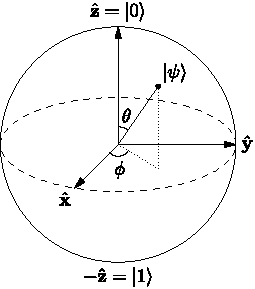
\includegraphics[scale=1.4]{images/Bloch_Sphere.pdf}
    \caption{Rappresentazione generale di un qubit sulla sfera di Bloch.}
    \label{fig:BlochSphere}
\end{figure}
\subsection{Matrice densità termica}
Supponiamo di avere $\hat \rho=\sum_n \omega_n \op{\psi_n}{\psi_n}$, in principio abbiamo molti modi per descrivere il nostro stato da $\ket{\psi_n}$ ognuno con probabilità $\omega_n$. Se il nostro sistema è libero di scambiare energia con l'ambiente abbiamo a che fare con un \textbf{sistema aperto}. Dopo un lungo periodo di tempo di interazione, il nostro sistema raggiungerà un equilibrio, cosicché la nostra probabilità per lo stato $\ket{\psi_n}$ sarà
\begin{equation*}
    \omega_n \equiv \frac{e^{-E_n/k_BT}}{Z} \, ,
\end{equation*}
dove $E_n$ è l'energia dello stato $\ket{\psi_n}$ e $Z=\sum_i e^{-E_i/k_BT}$ è la funzione di partizione canonica.\\
Se prendiamo la base $\ket n$ tale per cui $\hat H \ket n = E_n \ket n$ abbiamo
\begin{equation*}
    \hat \rho = \frac{e^{-\hat H/k_BT}}{Z}\, , \qquad Z=\Tr(e^{-\hat H/k_BT})=1\, , \qquad \rho_{mn}=\mel{m}{\hat \rho}{n}=\frac{e^{-E_n/k_BT}}{Z}\delta_{mn}\equiv \omega_n\, .
\end{equation*}
Usando la base computazionale $\{\ket 0, \ket 1\}$, con energie rispettivamente $E_0$, $E_1$, la matrice densità sarà
\begin{align*}
    \rho &= a_0 \op{0}{0} + a_1 \op{1}{1} \\
         &= \frac{e^{-E_0/k_BT}}{Z}\op{0}{0}+\frac{e^{-E_1/k_BT}}{Z}\op{1}{1}\, ,
\end{align*}
il rapporto tra i due coefficienti è pari a $a_1/a_0=e^{-\Delta E/k_BT}$ quindi possiamo osservare che se
\begin{itemize}
    \item $k_BT \gg \Delta E$, $a_1/a_0 \rightarrow 1$ la matrice densità è una miscela. Il sistema sarà portato allo stato massimamente miscelato (al centro della sfera di Bloch).
    \item $k_BT \ll \Delta E$, $a_1/a_0 \rightarrow 0$, $a_0 \rightarrow 1$ la matrice densità è uno stato puro, poiché il sistema disperde la sua energia nell'ambiente e decade nel suo stato fondamentale.
\end{itemize}
\section{Sistemi compositi}
Utilizziamo sistemi quantistici per studiarne i comportamenti quantistici, per farlo dobbiamo interagire con questi oggetti per misurare qualche loro proprietà, ad esempio sistemi macroscopici, come i rivelatori, interagiscono con sistemi microscopici. Dobbiamo trovare le connessioni che vi sono tra rivelatore e sistema. La terza componente che subentra tra rivelatore e sistema quantistico è l'ambiente, a differenza degli altri due, la sua trattazione è molto complessa per cui rimuoviamo l'ambiente e trattiamo il sistema composito rivelatore e sistema. \\
Trovando un modo di rimuovere l'ambiente dal nostro sistema composito, consideriamo due sistemi descritti rispettivamente da due spazi di Hilbert $\mathcal{H}_1$ e $\mathcal{H}_2$. Il sistema composito è dato da $\mathcal{H}_1\otimes\mathcal{H}_2=\mathcal{H}$. Se $\text{dim}\mathcal{H}_1 = n$ e $\text{dim}\mathcal{H}_2 = m$, allora $\text{dim}\mathcal{H} = n\times m$. Introduciamo l'ultimo postulato della meccanica quantistica
\begin{itemize}
    \item \textbf{V Postulato} (\textbf{Sistemi compositi}): Consideriamo un sistema quantistico composto da 2 sottosistemi $1$ e $2$ con spazi di Hilbert $\mathcal{H}_1$ e $\mathcal{H}_2$ rispettivamente. Lo spazio di Hilbert del sistema totale è dato da\footnote{Il simbolo "$\otimes$" indica il \textbf{prodotto tensoriale} tra spazi.} $\mathcal{H} = \mathcal{H}_1 \otimes \mathcal{H}_2$.
\end{itemize}
Se $\ket{\psi}_1\in\mathcal{H}_1$ e $\ket{\psi}_2\in\mathcal{H}_2$, allora $\ket{\psi}_1\otimes\ket{\psi}_2\in\mathcal{H}$, più precisamente se $\ket{n}_1$ e $\ket{m}_2$ sono una base per $\mathcal{H}_1$ e $\mathcal{H}_2$, allora $\ket{nm}$ è una base per $\mathcal{H}$. \\
Quando $n=m=2$, allora $\ket{nm}=\{\ket{00}, \ket{01}, \ket{10}, \ket{11}\}$ e $\ket \psi \in \mathcal{H}$ è scrivibile come $\ket{\psi}=\sum_{n,m}a_{nm}\ket{nm}$. \\
Introduciamo gli \textbf{stati separabili}, come suggerisce il nome si tratta di stati che possono essere trattati separatamente e si possono combinare le rispettive soluzioni in un secondo momento, infatti
\begin{equation*}
    \underbrace{\ket{\psi_1}}_{= \ket 0, \ket 1}\otimes\underbrace{\ket{\psi_2}}_{= \ket 0, \ket 1}=\alpha a \ket{00} + \alpha b \ket{01} + \beta a \ket{10} + \beta b \ket{11}
\end{equation*}
Accanto agli stati, abbiamo gli operatori che lavorano in questo spazio $\mathcal{H}$, per esempio se $\hat A \in L(\mathcal{H}_1)$, $\hat B \in L(\mathcal{H}_1)$, allora $\hat U = \hat A \otimes \hat B$. Quest'ultimo operatore agisce nel seguente modo
\begin{equation*}
    \hat U \ket \psi = \hat A \otimes \hat B(\ket{\psi_1}\otimes\ket{\psi_2})=\hat A\ket{\psi_1}\otimes \hat B\ket{\psi_2}
\end{equation*}
Perché ci interessa? Perché questi operatori possono essere associati ad osservabili! Come realizziamo una misura su un sistema composito? Supponiamo di avere
\begin{equation*}
    \tilde{A}=A\otimes \mathbb{I} \Rightarrow \tilde{A}: \mathcal{H} \rightarrow \mathcal{H}
\end{equation*}
$\hat A$ rappresenta la misura su un sistema di qubit mentre $\hat B$ l'identità. In questo caso $\hat A$ possiede due proiettori
\begin{equation*}
    P_A^0 = \op{0}{0} \qquad P_A^1=\op{1}{1} \, ,
\end{equation*}
e vogliamo andare a valutare
\begin{equation*}
    \expval{\tilde{A}}=\expval{A\otimes \mathbb{I}}=\mel{\psi}{A \otimes \mathbb{I}}{\psi}=\sum_{ijk}a_{ij}^*a_{kj}\mel{i}{A}{k} \, ,
\end{equation*}
dove ovviamente $\ket \psi \in \mathcal{H}, \ket \psi = \sum_{ij}a_{ij}\ket{ij}$.\\
Otteniamo così
\begin{equation*}
    \expval{\tilde{A}}=\sum_{ij}a_{ij}^2\mel{i}{A}{j} \, .
\end{equation*}
La funzione d'onda che andiamo a considerare è data da $\ket{\psi_1}\otimes\ket{\psi_2}$ e risulta essere definita come
\begin{equation*}
    \ket \psi = \alpha a \ket{00} + \alpha b \ket{01} + \beta a \ket{10} + \beta b \ket{11}\, ,
\end{equation*}
da cui otteniamo che
\begin{align*}
    &\hat A \ket 0 = \ket 0 \\
    &\hat A \ket 1 = -\ket 1 
\end{align*}
cioè
\begin{equation*}
    \hat A = \begin{pmatrix}1 & 0 \\ 0 & -1 \end{pmatrix}
\end{equation*}
e il suo valore di aspettazione è pari a
\begin{equation*}
    \expval{A}=(\alpha a)^2 + (\alpha b)^2 - (\beta a)^2 - (\beta b)^2 \, .
\end{equation*}
Nel caso in cui
\begin{align*}
    &A\otimes\mathbb{I}\left[\frac{\ket{00}+\ket{01}}{\sqrt 2}\right] \Rightarrow \ket{00}, \ket{01} \quad \text{sono stati separabili} \\
    &A\otimes\mathbb{I}\left[\frac{\ket{01}-\ket{10}}{\sqrt 2}\right] \Rightarrow \ket{01}, \ket{10} \quad \text{sono stati entangled} \\
\end{align*}
\subsection{Matrice densità ridotta}
Se abbiamo uno spazio di Hilbert $\mathcal{H}_A$ e misuriamo l'osservabile $\hat A$ ($a_k$, $\ket{a_k}$, abbiamo una probabilità di ottenere il risultato $a_k$ pari a
\begin{equation*}
    p(a_k)=\Tr\left(\op{a_k}{a_k}\rho\right)=\Tr\left(P_{a_k}\rho\right) \, .
\end{equation*}
Altre informazioni che possiamo ottenere sono
\begin{equation*}
    \expval{A}=\Tr(A\rho) \, ,
\end{equation*}
dove
\begin{equation*}
    \rho \rightarrow \frac{P_{a_k}\rho P_{a_k}}{\sqrt{\Tr{P_{a_k}\rho}}} \, ,
\end{equation*}
questo discorso è valido per un qubit. Supponiamo di considerare ora un qubit connesso a un rivelatore, ambiente, \dots In questo caso lo spazio di Hilbert è dato da $\mathcal{H}_A \otimes \mathcal{H}_B$, in questo caso la matrice densità $\rho^{AB}$ è un operatore appartenere a questo spazio. Vogliamo sapere se possiamo ottenere informazioni sul sottospazio $\mathcal{H}_A$, ignorando completamente $\mathcal{H}_B$, la risposta è affermativa e lo si fa nel seguente modo
\begin{equation*}
    \rho^A = \Tr_B(\rho^{AB}) \, ,
\end{equation*}
questa quantità prende il nome di \textbf{matrice densità ridotta}. Cerchiamo di formalizzare meglio questo risultato. \\
Siano $A:\mathcal{H}_A \rightarrow \mathcal{H}_A$ e $B:\mathcal{H}_B \rightarrow \mathcal{H}_B$ due operatori. La loro combinazione è definita come $A \otimes B:\mathcal{H}_A\otimes \mathcal{H}_B \rightarrow \mathcal{H}_A\otimes\mathcal{H}_B$, la \textbf{traccia parziale} è data da
\begin{align*}
    &\Tr_A : L(\mathcal{H}_A\otimes \mathcal{H}_B) \rightarrow L(\mathcal{H_B}) \\
    &\Tr_B : L(\mathcal{H}_A\otimes \mathcal{H}_B) \rightarrow L(\mathcal{H_A}) \, .
\end{align*}
Consideriamo il seguente esempio
\begin{esempio}
Sia $\rho^{AB}=\rho \otimes \sigma$, vogliamo valutare la traccia parziale sul sottospazio $\mathcal{B}$, in questo caso
\begin{equation*}
    \rho^A = \Tr_B(\rho^{AB})=\Tr_B(\rho \otimes \sigma)=\Tr(\sigma)\rho = \rho
\end{equation*}
questo per quanto riguarda \textbf{stati separabili}, ma in generale non è sempre vero! Infatti supponiamo di considerare
\begin{equation*}
    \rho = \frac{\ket{00}+\ket{11}}{\sqrt 2}\frac{\bra{00}+\bra{11}}{\sqrt 2}
\end{equation*}
se eseguissimo la traccia parziale sul sottospazio $\mathcal{H}_2$, avremmo che
\begin{equation*}
    \rho_1 = \Tr_2\rho = \frac{\mathbb{I}}{2}
\end{equation*}
In questo caso, abbiamo sì che $\Tr (\rho_1)=1$, ma $\Tr(\rho_1^2)=\frac 12$, cioè $\rho_1$ è una miscela di stati!
\end{esempio}
    \vspace{0.5cm}
\noindent \lecture{5}{21/10/2021}

\section{Interazione con l'ambiente}

Consideriamo un qubit interagire con l'ambiente. Essendo il qubit un sistema non chiuso, non possiamo descrivere la sua evoluzione temporale come sola evoluzione del qubit. Bisognerà allora tenere in conto della sua interazione con l'ambiente e per farlo possiamo sfruttare la \textbf{matrice densità}. L'equazione del moto per la matrice densità, chiamata \textbf{equazione di Liouville-von Neumann}, segue direttamente dall'equazione di Schrödinger:
\begin{equation}
    \dv{\hat \rho}{t} = \sum_j \dv{t} \left(p_j\op{\psi_j}{\psi_j}\right)=\sum_j p_j\frac{1}{i\hbar}\left(\hat H \op{\psi_j}{\psi_j}-\op{\psi_j}{\psi_j}\hat H\right)=\frac{1}{i\hbar}\comm{\hat H}{\hat \rho} \, .
    \label{eq:liouville-von-neumann}
\end{equation}
L'evoluzione descritta dall'equazione \eqref{eq:liouville-von-neumann} è unitaria e la sua soluzione può essere scritta come
\begin{equation*}
    \hat \rho (t) = \hat U(t)\hat \rho(0) \hat U^\dagger(t) \, .
\end{equation*}
Tuttavia, questo processo descritto dalla \eqref{eq:liouville-von-neumann} non descrive alcun cambiamento sulla sua purezza, infatti quest'ultima risulta essere preservata:
\begin{equation*}
    \hat \xi(t) = \Tr\left(\hat \rho(t)^2\right) = \Tr\left(\hat U(t)\hat \rho(0) \hat U^\dagger(t)\hat U(t)\hat \rho(0) \hat U^\dagger(t)\right)=\Tr\left(\hat \rho (0)^2\right)=\hat \xi(0)
\end{equation*}
Questo significa che l'evoluzione di uno stato pure in una miscela di stati, includendo il processo di misurazione, non può essere descritto dalla \eqref{eq:liouville-von-neumann} ed è un processo essenzialmente non unitario.\\
Per risolvere questo aspetto l'hamiltoniana deve includere più termini
\begin{equation*}
    \hat H = \hat H_S + \hat H_E + \hat H_I \, ,
\end{equation*}
essi sono rispettivamente l'hamiltoniana di sistema, dell'ambiente e di interazione tra sistema e ambiente. Se assumiamo, come è ragionevole, che il sistema non abbia alcun effetto sull'ambiente e che l'hamiltoniana di interazione sia piccola (e quindi possiamo trattarla con la teoria perturbativa) possiamo facilmente studiare l'evoluzione della matrice densità nella rappresentazione d'interazione
\begin{equation*}
    \dv{\hat \rho_{int}}{t}=\frac{1}{i\hbar}\comm{\hat H_{int\,I}(t)}{\hat \rho_{int}(t)} \, ,
\end{equation*}
e
\begin{equation*}
    \hat \rho(t) = \hat \rho (-\infty) + \frac{1}{i\hbar}\int_{-\infty}^t \dd{t'}\comm{\hat H_{I}(t')}{\hat \rho(t')} \, ,
\end{equation*}
dove, supponendo che non solo inizialmente il sistema e l'ambiente fossero statisticamente indipendenti l'uno dall'altro, ma rimarranno tali, possiamo scrivere
\begin{align*}
    \hat \rho(-\infty) &= \hat \rho_S(-\infty)\otimes\hat\rho_E \\
    \hat \rho (t) &= \hat \rho_S(t)\otimes\hat\rho_E \, .
\end{align*}
A questo punto, possiamo tracciare la matrice densità sull'ambiente e ottenere una matrice densità ridotta per il sistema
\begin{equation*}
    \Tr_E\hat \rho(t) = \hat \rho_S(t)
\end{equation*}
Tornando alla rappresentazione di Schrödinger, svolgendo un paio di conti e assunzioni che non stiamo qui a discutere, otteniamo una \textbf{master equation} nella forma di \textbf{Lindblad}

\begin{equation}
    \dv{\hat\rho}{t} = \frac {1}{i\hbar} [\hat H, \hat \rho] + \sum_a \left( 2L_a \hat \rho L_a^\dagger - L_a^\dagger L_a\hat \rho - \hat \rho L_a^\dagger L_a\right)
    \label{eq:master}
\end{equation}
Cosa rende l'equazione \eqref{eq:master} così importante è il fatto che modelli l'evoluzione non unitaria della matrice densità del sistema. Lo stesso comportamento non potrebbe essere descritto dalla nostra equazione iniziale \eqref{eq:liouville-von-neumann} per l'intero insieme: sistema più ambiente.

\begin{esempio}[Evoluzione non unitaria di un qubit: rilassamento e sfasamento]
Supponiamo di considerare un sistema i cui stati siano $\ket 0$ e $\ket 1$. L'hamiltoniana di riferimento per questo sistema è
\begin{equation*}
    \hat H_S = \begin{pmatrix}E_0 & 0 \\ 0 & E_1\end{pmatrix}
\end{equation*}
Utilizzando la rappresentazione di interazione, possiamo scrivere la \textbf{master equation} come
\begin{equation}
        \dv{\hat\rho}{t} = \sum_a \left( 2L_a \hat \rho L_a^\dagger - L_a^\dagger L_a\hat \rho - \hat \rho L_a^\dagger L_a\right)
        \label{eq:master-example}
\end{equation}
a questo punto possiamo considerare i primi tre termini degli \textit{operatori di Lindblad}:
\begin{align*}
    & L_1 =L_1^\dagger =\sqrt \gamma \sigma_+\sigma_-=\sqrt\gamma\begin{pmatrix}1 & 0\\ 0 & 0\end{pmatrix}\\
    & L_2 = \sqrt{\frac{\Gamma}{2}}\sigma_- = \sqrt{\frac{\Gamma}{2}}\begin{pmatrix}0 & 0\\ 1 & 0\end{pmatrix} \\
    & L_2^\dagger = \sqrt{\frac{\Gamma}{2}}\sigma_+ = \sqrt{\frac{\Gamma}{2}}\begin{pmatrix}0 & 1\\ 0 & 0\end{pmatrix} \\
    & L_3 = \sqrt{\frac{\Gamma}{2}}\sigma_+ = \sqrt{\frac{\Gamma}{2}}\begin{pmatrix}0 & 1\\ 0 & 0\end{pmatrix} \\
    & L_3^\dagger = \sqrt{\frac{\Gamma}{2}}\sigma_- = \sqrt{\frac{\Gamma}{2}}\begin{pmatrix}0 & 0\\ 1 & 0\end{pmatrix}
\end{align*}
Sostituendo il primo in \eqref{eq:master-example} otteniamo
\begin{equation*}
    \dv{\hat\rho}{t} = \begin{pmatrix}0 & -\gamma\rho_{01}\\-\gamma\rho_{10} & 0\end{pmatrix}
\end{equation*}
che integrata
\begin{equation*}
    \hat \rho(t) = \begin{pmatrix}\rho_{00}(0) & \rho_{01}(0)e^{-\gamma t} \\ \rho_{10}(0)e^{-\gamma t} & \rho_{11}(0) \end{pmatrix}
\end{equation*}
I termini diagonali non vengono affatto modificati, quindi questa scelta di $L_1$ realizza quello che viene chiamato uno \textbf{sfasamento}. L'equazione ottenuta può essere considerata come un modello del processo di misura, in cui lo stato $\ket 0$ o $\ket 1$ del sistema è osservato, con $\tau_\gamma = 1/\gamma$ che fornisce il tasso di collasso dello stato.\\
Per quanto riguarda $L_2^\dagger$ ed $L_3$, otteniamo
\begin{equation*}
    \dv{\hat\rho}{t} = \begin{pmatrix}-\Gamma\rho_{00} & -(\Gamma/2)\rho_{01}\\-(\Gamma/2)\rho_{10} & \Gamma\rho_{00}\end{pmatrix}
\end{equation*}
con soluzione
\begin{equation*}
    \hat \rho(t) = \begin{pmatrix}\rho_{00}(0)e^{-\Gamma t} & \rho_{01}(0)e^{-(\Gamma/2)t} \\ \rho_{10}(0)e^{-(\Gamma/2) t} & 1-\rho_{00}(0)e^{-\Gamma t} \end{pmatrix}
\end{equation*}
e in maniera simile per $L_2$ e $L_3^\dagger$
\begin{equation*}
        \dv{\hat\rho}{t} = \begin{pmatrix} \Gamma\rho_{11} & -(\Gamma/2)\rho_{01}\\-(\Gamma/2)\rho_{10} & -\Gamma\rho_{11}\end{pmatrix}
\end{equation*}
con soluzione
\begin{equation*}
    \hat \rho(t) = \begin{pmatrix}1-\rho_{11}(0)e^{-\Gamma t} & \rho_{01}(0)e^{-(\Gamma/2)t} \\ \rho_{10}(0)e^{-(\Gamma/2) t} & \rho_{11}(0)e^{-\Gamma t} \end{pmatrix}
\end{equation*}
Oltre allo \textbf{sfasamento}, queste equazioni mostrano anche il \textbf{rilassamento} o \textbf{eccitamento} degli elementi diagonali. Fisicamente, ciò significa che Lindblads $L_2$, $L_3$ descrivono i processi concorrenti di trasmissione di energia tra il sistema e l'ambiente. Si noti che l'evoluzione delle matrici densità ricavate portano infine a uno stato puro, a un autostato dell'hamiltoniana del sistema. Affinché il sistema si rilassi in uno stato misto, l'equazione principale deve includere entrambi i termini che indicano uno \textbf{sfasamento} e un'\textbf{eccitazione} o \textbf{rilassamento}, con pesi appropriati. Se includiamo tutte gli operatori di Lindblad, la soluzione dell'equazione principale avrà la forma
\begin{equation*}
    \hat \rho(t) =
    \begin{pmatrix}
        \overline{\rho_{00}} + (\rho_{00}(0)-\overline{\rho_{00}})e^{-\Gamma t} & \overline{\rho_{01}}(0)e^{-(\Gamma/2+\gamma) t} \\
        \overline{\rho_{10}}(0)e^{-(\Gamma/2+\gamma) t} &
        \overline{\rho_{11}} + (\rho_{11}(0)-\overline{\rho_{11}})e^{-\Gamma t}
    \end{pmatrix}
\end{equation*}
dove i valori stazionari $\overline{\rho_{00}}+\overline{\rho_{11}}=\rho_{00}(0)+\rho_{11}(0)=1$ sono le eventuali probabilità di occupazione dei livelli. Se il sistema si rilassa verso l'equilibrio ad una certa temperatura, allora $\rho_{11}/\rho_{00} = \exp[-(E_1-E_0)/k_BT]$,
\end{esempio}
\noindent In questo contesto possiamo definire il \textbf{tempo di coerenza}, che risulta essere caratterizzato da:
\begin{itemize}
    \item \textbf{Relaxation time}: $\frac{1}{T_1}=\frac{\Gamma}{2}$
    \item \textbf{Dephasing time}: $\frac{1}{T_2}=\frac{\Gamma}{2} + \gamma$
\end{itemize}
Quando si realizza un qubit, è importante andare a misurare $T_1$ e $T_2$, così da caratterizzare al meglio il nostro sistema a due livelli.

\chapter{Misurazioni}
Abbiamo già introdotto il concetto di misura proiettiva e di misura a valori operatoriali positivi, ma avevamo sempre immaginato di agire su un grande insieme di stati uguali. Al contrario, adesso, ci concentreremo su misure di singoli oggetti, come può essere un qubit.
Lo strumento per misurare un singolo oggetto è, chiaramente, il fotone. Dal momento che esso può essere descritto sia come particella che come onda, più o meno localizzata, potremo studiarne la dispersione tramite il principio di indeterminazione di Heisenberg:

\begin{definizione}[\textbf{Principio di indeterminazione di Heisenberg}]
    Dati due osservabili $\hat A$ e $\hat B$, il valore d'aspettazione della deviazione standard degli stessi su di un particolare stato $\ket \psi$ è limitato dalla relazione:
    
    \begin{equation}
        \Delta A \Delta B \geq \frac{1}{2}\bra \psi \comm{A}{B} \ket \psi
    \end{equation}
\end{definizione}
\noindent Da questa equazione possiamo ricavare:
\begin{equation*}
    \Delta x \Delta p \geq \frac{\hbar}{2}
\end{equation*}
Spesso viene scritta e associata al principio di indeterminazione anche una \textbf{relazione di indeterminazione energia-tempo} che, tuttavia, non rientra nella casistica prevista dal principio di indeterminazione di Heisenberg (poiché non esiste alcun operatore "tempo").
\begin{equation*}
    \Delta E \Delta t \geq \frac{\hbar}{2}
\end{equation*}
Le relazioni che abbiamo scritto fino ad ora descrivono limiti intrinseci nella preparazione dei sistemi quantistici, ma sono chiaramente connessi a un'incertezza relativa alle misurazioni.
Vediamo ora un esempio per mostrare il collegamento fra incertezza nella preparazione e incertezza nella misura.

\section{Microscopio di Heisenberg}

\textbf{Microscopio di Heisenberg:}
Immaginiamo di avere un elettrone di cui vogliamo misurare la posizione. Abbiamo bisogno di almeno un fotone per visualizzare l'elettrone e dobbiamo fare in modo che esso sia deflesso dall'elettrone all'interno del cono ad angolo $\theta$ (in modo da incidere sulla lente del nostro microscopio).

\begin{wrapfigure}{r}{4cm}
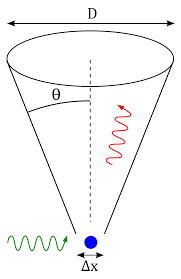
\includegraphics[width=3.5cm]{images/heisenberg_microscope.png}
\caption{Esperimento pensato del microscopio di Heisenberg.}\label{img-heisenberg_microscope}
\end{wrapfigure} 
\noindent A seconda dell'angolo di scattering dell'elettrone esso acquisirà un momento (più alta sarà l'energia del fotone più alto sarà il momento finale dell'elettrone).
Abbiamo quindi quella che viene chiamata \textbf{back action}: misurando un oggetto quantistico tramite un altro oggetto quantistico abbiamo influenzato e modificato il sistema stesso.
L'ottica classica ci fornisce una legge di diffrazione tale per cui:
\begin{equation*}
    \sin \theta \approx \frac{\lambda}{D}
\end{equation*}
Siccome il fotone è un'onda, il microscopio arriva a ottenere la posizione dell'elettrone con un'incertezza $\Delta x = \frac{\lambda}{\sin \theta}$ per cui si avrà:
\begin{equation*}
    -\frac{h}{\lambda}\sin \theta \le p_x \le \frac{h}{\lambda}\sin \theta
\end{equation*}
Da cui discende direttamente che: $\Delta p_x = \frac{2 h}{\lambda}\sin \theta$.
Dunque se voglio misurare solamente la posizione posso modificare $\lambda$ per avere una precisione arbitraria, ma non posso misurare in contemporanea il momento poiché:
\begin{equation*}
    \Delta p_x \Delta x = h
\end{equation*}
Che è una relazione evidentemente molto simile a quella ricavata dal principio di indeterminazione di Heisenberg: un'incertezza "alla Heisenberg" sulla sonda (il nostro fotone) ci porta a una necessaria incertezza sull'osservabile finale.
    %%%%%%%%%%%%%
% LECTURE 6 %
%%%%%%%%%%%%%

\vspace{1cm}

\noindent \lecture{6}{22/10/2021}

\section{Quantum Parallelism}

\begin{definizione}[\textbf{Quantum Parallelism}]
    Il \textbf{quantum parallelism} è una delle caratteristiche fondamentali di molti algoritmi quantistici. Consente ai computer quantistici di valutare una funzione $f(x)$ per molti valori diversi di $x$ contemporaneamente.
\end{definizione}
\noindent Supponiamo di considerare la più semplice funzione possibile $f(x):\{0,1\}^{\otimes n} \rightarrow \{0,1\}$ definita su un dominio (insieme di numeri costruiti con $n$ cifre di 0 e 1) e a elementi in un intervallo di bit. Assumiamo inoltre si saper calcolare efficientemente nel nostro computer tale funzione. Ciò che calcoliamo, dal punto di vista della computazione classica, lo possiamo valutare nella computazione quantistica, pertanto tutte le operazioni aritmetiche possono essere svolte dal calcolo quantistico. Un modo quindi di calcolare questa funzione su un computer quantistico è quello di considerare due differenti stati: immaginiamo un qubit $\ket{y}$ e uno stato che può essere un prodotto tensoriale di qubit, come ad esempio $\ket{0}^{\otimes n}$. Spesso considereremo lo stato $\ket{0}^{\otimes n}$ come stato iniziale in cui il computer quantistico viene preparato mediante una misurazione nella base computazionale perché è facilmente costruibile: ad esempio nel caso $n=3$ se, a seguito di una misurazione, lo stato nel QC collassa in $\ket{\psi} \rightarrow \ket{1} \otimes \ket{0} \otimes \ket{1}$, basterà applicare un \texttt{X-gate} al primo e al terzo qubit per costruire lo stato voluto $\ket{0}^{\otimes 3}$.

\noindent Chiamiamo lo stato iniziale totale $\ket{x,y}$, dove $x$ contiene l'informazione iniziale data in input e $y$ conterrà, dopo delle opportune operazioni, il risultato cercato. Con un'appropriata sequenza di gate è possibile effettuare la trasformazione
\begin{equation}\label{black_box_U_f}
    \ket{x,y} \overset{U_f}{\longrightarrow} \ket{x,y \oplus f(x)} \, ,
\end{equation}
dove $U_f$ è un opportuno gate unitario che implementa l'operazione desiderata. Il circuito che implementa la \eqref{black_box_U_f} è 
\begin{center}
    \mbox{
        \Qcircuit @C=1em @R=1em {
            \lstick{\ket{x}} & \multigate{1}{U_f} & \rstick{\ket{x}} \qw \\
            \lstick{\ket{y}} & \ghost{U_f} & \rstick{\ket{y\oplus f(x)}} \qw
        }
    }
\end{center}
dove $\ket{x}$ prende il nome di \textbf{data register} e $\ket{y}$ prende il nome di \textbf{target register}. Questa rappresentazione è utile perché quando $\ket{y} = \ket{0}$ l'output del target register è esattamente l'oggetto che si vuole calcolare
\begin{center}
    \mbox{
        \Qcircuit @C=1em @R=1em {
            \lstick{\ket{x}} & \multigate{1}{U_f} & \rstick{\ket{x}} \qw \\
            \lstick{\ket{0}} & \ghost{U_f} & \rstick{\ket{0\oplus f(x)}=\ket{f(x)}} \qw
        }
    }
\end{center}
Notiamo che la \eqref{black_box_U_f} è invertibile: se applichiamo $U_f$ due volte, otteniamo:
\begin{equation*}
    \ket{x,y} \rightarrow \ket{x, y \oplus f(x)} \rightarrow \ket{x,y \oplus f(x) \oplus f(x)} = \ket{x,y} \, ,
\end{equation*}
siccome $f(x) \oplus f(x) = 0$ indipendentemente dai valori di $f$. Fino ad ora avremmo potuto effettuare tutte queste operazioni in CC. L'importanza del QC risiede nel fatto che si possano considerare sovrapposizioni di stati appartenenti ad una base. Consideriamo il caso $n = 1$ (il data register è un qubit) e assumiamo il seguente stato iniziale
\begin{equation*}
    \ket{x,y} \equiv \underbrace{\frac{1}{\sqrt 2} (\ket{0}+\ket{1})}_{\ket{x}} \otimes \underbrace{\ket 0}_{\ket{y}} = \frac{1}{\sqrt 2} \left( \ket{00}+\ket{10} \right) \, ;
\end{equation*}
Se assumiamo che il computer sia preparato in $\ket{0} \otimes \ket{0}$ come possiamo rappresentare $\ket{x,y}$ in un circuito ? Possiamo sfruttare l'\texttt{H-gate} in questo modo:
\begin{center}
    \mbox{
        \Qcircuit @C=1em @R=1em {
            \lstick{\ket{0}} & \gate{H} & \multigate{1}{U_f} & \qw \\
            \lstick{\ket{0}} & \qw & \ghost{U_f} & \qw
            %\gategroup{1}{4}{2}{4}{0.8em}{\}}
        }
    }
\end{center}
infatti, utilizzando la \eqref{black_box_U_f}, avremo
\begin{equation*}
    \ket{0,0} \overset{H}{\longrightarrow} \frac{1}{\sqrt{2}} \left( \ket{00}+\ket{10} \right) \overset{U_f}{\longrightarrow} \frac{1}{\sqrt{2}} \left( \ket{0, f(0)} + \ket{1, f(1)} \right) \, .
\end{equation*}
Questo circuito è particolarmente interessante perché l'output è una sovrapposizione di differenti stati contenenti informazioni riguardo la funzione: $f(0)$ e $f(1)$ appaiono simultaneamente nel medesimo stato. È come se avessimo valutato $f(x)$ per due valori di $x$ contemporaneamente, parallelamente! A differenza del classic parallelism, in cui più circuiti vengono costruiti per calcolare $f(x)$ ed eseguiti simultaneamente, qui viene impiegato un singolo circuito per valutare la funzione $f(x)$ per più valori di $x$ nello stesso momento: si sta sfruttando la capacità di un computer quantistico di essere in sovrapposizioni di stati diversi. Qui risiede il \textbf{quantum parallelism}.

\noindent Questo discorso può essere facilmente generalizzato al caso di $n$-qubit. Supponiamo che il data register si trovi in $\ket{0}^{\otimes n}$. Usiamo il fatto che l'azione dell'\texttt{H-gate} su $n$-qubit possa essere scritta nel seguente modo:
\begin{align}
    H^{\otimes n}\ket{0}^{\otimes n} &= \underbrace{H\otimes \cdots \otimes H}_{n\text{-volte}} \underbrace{\ket{0} \otimes \cdots \otimes \ket{0}}_{n\text{-volte}} = \frac{1}{\sqrt 2} (\ket 0 + \ket 1) \otimes \cdots \otimes \frac{1}{\sqrt 2} (\ket 0 + \ket 1) \notag \\
    &= \frac{1}{\sqrt{2^n}}(\ket{000 \ldots 0} + \ket{010 \ldots 0} + \ldots + \ket{111 \dots 1}) = \frac{1}{\sqrt{2^n}}\sum_{x=0}^{2^n-1}\ket{x} \, , \label{n_H_gates}
\end{align}
dove $x$ rappresenta tutte le possibili stringhe di $n$-volte $0$ e $1$. Se il target si trova in $\ket{y} = \ket{0}$ e applichiamo ora $U_f$, il risultato è:
\begin{equation*}
    \frac{1}{\sqrt{2^n}}\sum_{x=0}^{2^n-1}\ket{x} \otimes \ket{0} \overset{U_f}{\longrightarrow} \frac{1}{\sqrt{2^n}}\sum_{x=0}^{2^n-1}\ket{x,f(x)} \, ,
\end{equation*}
dove si è fatto uso della \eqref{black_box_U_f} con $\ket{y} = \ket{0}$. In termini di circuiti avremo
\begin{center}
    \mbox{
        \Qcircuit @C=1em @R=1em {
            \lstick{\ket{0}^{\otimes n}} & \gate{H^{\otimes n}} & \multigate{1}{U_f} & \qw & \qw \\
            \lstick{\ket{y} = \ket{0}} & \qw & \ghost{U_f}   & \qw      & \qw
        }
    }
\end{center}
In un certo senso, il quantum parallelism consente di valutare simultaneamente tutti i possibili valori della funzione $f(x)$, anche se apparentemente abbiamo valutato $f(x)$ in una singola volta. Precisiamo che la misura dello stato nel caso del qubit singolo ci darà solamente $\ket{0, f(0)}$ oppure $\ket{1, f(1)}$. In maniera analoga per il caso generale, la misura dello stato $\sum_x\ket{x,f(x)}$ ci darà un solo $f(x_0)$ per un singolo valore casuale $x_0$. Ovviamente un computer classico può farlo più facilmente! La computazione quantistica richiede qualcosa di più del semplice quantum parallelism per essere utile; richiede cioè la capacità di estrarre informazioni su più di un valore di $f(x)$ da stati di sovrapposizione, come $\sum_x\ket{x,f(x)}$. Come vedremo nella prossima sezione, il "trucco" di considerare una sovrapposizione lineare ci permetterà di estrarre alcune informazioni su $f$ in un modo più efficiente del CC.

\section{Algoritmo di Deutsch}
Una semplice modifica del circuito precedente dimostra come i circuiti quantistici possano essere più performanti rispetto a quelli classici. Nelle ultime righe del paragrafo precedente abbiamo detto che la computazione quantistica richiede qualcosa di più oltre al quantum parallelism per essere utilizzabile. L'\textbf{algoritmo di Deutsch} combina il meccanismo del \textbf{quantum parallelism} con la proprietà della meccanica quantistica dell'\textbf{interferenza}. 

\noindent Si tratta di un algoritmo un po' accademico (le funzioni sono banali), tuttavia utile per illustrare l'idea di algoritmo quantistico. Lasciamo che entrambi input e output register contengano ciascuno un solo qubit, quindi stiamo esplorando le funzioni $f(x)$ che convertono un singolo bit in un singolo bit: $f(x): \; \{ 0,1 \} \rightarrow \{ 0,1 \}$. Ci sono due modi piuttosto diversi di pensare a tali funzioni. Il primo modo è notare che ci sono solo quattro di queste funzioni, come mostrato nella Tabella \ref{tab:Deutsch_Fnct}.

\begin{table}[!ht]
	\centering
    \begin{tabular}{ccc}
        \toprule
        & $x = 0$ & $x=1$ \\
        \midrule
        $f_0$ & $0$ & $0$ \\
        $f_1$ & $0$ & $1$ \\
        $f_2$ & $1$ & $0$ \\
        $f_3$ & $1$ & $1$ \\
        \bottomrule
    \end{tabular} \\
    \caption{Esistono solo quattro funzioni distinte $f_j(x)$ che convertono un bit in un bit, tutte facilmente implementabili sia in un computer classico che quantistico.}
    \label{tab:Deutsch_Fnct}
\end{table}

\noindent Supponiamo che ci venga data una black-box (ossia un gate ignoto che indicheremo con \texttt{U-gate}) che calcola una di queste quattro funzioni eseguendo la seguente trasformazione unitaria:
\begin{equation*}
    U_{f_j} \ket{x,y} = \ket{x, y \oplus f_j(x)} \, .
\end{equation*}
In questo caso, se implementiamo in circuiti la Tabella \ref{tab:Deutsch_Fnct} avremo:

\begin{center}
    \mbox{
        $
        \begin{matrix}
             \\
             \\
            f_0: \\
        \end{matrix}
        $
        \Qcircuit @C=1em @R=1em {
            & \multigate{1}{U_{f_0}} & \qw \\
            & \ghost{U_{f_0}}& \qw \\
        }
        $
        \begin{matrix}
             \\
             \\
            \ = \\
        \end{matrix}
        $
        \Qcircuit @C=1em @R=1.9em {
            & \qw & \qw & \qw & \qw & \qw \\
            & \qw & \qw & \qw & \qw & \qw \\
        }
    }
    \qquad \qquad
    \mbox{
        $
        \begin{matrix}
             \\
             \\
            f_1: \\
        \end{matrix}
        $
        \Qcircuit @C=1em @R=1em {
            & \multigate{1}{U_{f_1}} & \qw \\
            & \ghost{U_{f_1}}& \qw \\
        }
        $
        \begin{matrix}
             \\
             \\
            \ = \\
        \end{matrix}
        $
        \Qcircuit @C=1em @R=1.35em {
            & \ctrl{1} & \qw & \qw \\
            & \targ & \qw & \qw  \\
        }
    }
\end{center}
\begin{center}
    \mbox{
        $
        \begin{matrix}
             \\
             \\
            f_2: \\
        \end{matrix}
        $
        \Qcircuit @C=1em @R=1em {
            & \multigate{1}{U_{f_2}} & \qw \\
            & \ghost{U_{f_2}}& \qw \\
        }
        $
        \begin{matrix}
             \\
             \\
            \ = \\
        \end{matrix}
        $
        \Qcircuit @C=1em @R=1.15em {
            & \qw & \ctrl{1} & \qw \\
            & \gate{X} & \targ & \qw \\
        }
    }
    \qquad \qquad
    \mbox{
        $
        \begin{matrix}
             \\
             \\
            f_3: \\
        \end{matrix}
        $
        \Qcircuit @C=1em @R=1em {
            & \multigate{1}{U_{f_3}} & \qw \\
            & \ghost{U_{f_3}}& \qw \\
        }
        $
        \begin{matrix}
             \\
             \\
            \ = \\
        \end{matrix}
        $
        \Qcircuit @C=1em @R=1.25em {
            & \qw & \qw \\
            & \gate{X} & \qw \\
        }
    }
\end{center}
Dato che la regola che vogliamo implementare è $\ket{x,0} \rightarrow \ket{x, f(x)}$ ($\ket{y}$ inizializzato a $\ket{0}$), in termini matematici questo significa scrivere:
\begin{align*}
    &f_0: &\ket{x,0} &\longrightarrow \ket{x,0} \, , \\
    &f_1: &\ket{x,0} &\overset{\texttt{CNOT}}{\longrightarrow} 
    \begin{cases}
        \ket{0,0} \, , &\text{per } x = 0 \\
        \ket{1,1} \, , &\text{per } x = 1
    \end{cases} \, , \\
    &f_2: &\ket{x,0} &\overset{X}{\longrightarrow} \ket{x,1} \overset{\texttt{CNOT}}{\longrightarrow}
    \begin{cases}
        \ket{0,1} \, , &\text{per } x = 0 \\
        \ket{1,0} \, , &\text{per } x = 1
    \end{cases} \, , \\
    &f_3: &\ket{x,0} &\overset{X}{\longrightarrow} \ket{x,1} \, , 
\end{align*}

\noindent Supponiamo che ci venga data una black-box che esegua $U_f$ per una delle quattro funzioni, ma non ci venga detto quale delle quattro operazioni. Ovviamente possiamo scoprirlo lasciando agire due volte la black-box, prima su $\ket0 \otimes \ket0$ e poi su $\ket 1 \otimes \ket 0$. Ma supponiamo di poter far agire la black-box solo una volta. Cosa possiamo conoscere di $f(x)$ ?

\noindent In un computer classico, dove siamo effettivamente limitati a lasciare che la black-box agisca sui qubit in uno dei quattro stati di base computazionale, possiamo conoscere il valore di:
\begin{itemize}
    \item $f(0)$, lasciando che $U_f$ agisca su uno dei due $\ket0 \otimes \ket0$ o $\ket0 \otimes \ket1$;
    \begin{itemize}
        \item In tal caso possiamo limitare la scelta a $f_0$ o $f_1$ (se $f(0) = 0$) oppure $f_2$ o $f_3$ (se $f(0) = 1$).
    \end{itemize}
    \item $f(1)$, lasciando che $U_f$ agisca su $\ket1 \otimes \ket0$ o $\ket1 \otimes \ket1$;
    \begin{itemize}
        \item In questa situazione abbiamo ristretto la funzione ad essere $f_0$ o $f_2$ (se $f(1) = 0$) oppure $f_1$ o $f_3$ (se $f(1) = 1$).
    \end{itemize}
\end{itemize}
In definitiva, un computer classico necessita di due esecuzioni per determinare se $f$ sia costante o meno. Sorprendentemente, risulta che con un computer quantistico questo non è necessario perché il problema può essere risolto con una singola esecuzione. Il punto interessante è che l'algoritmo non riguarda il calcolo preciso della funzione, ma piuttosto la comprensione di una o più sue proprietà: quando l'algoritmo viene lanciato non impariamo nulla sui valori individuali di $f(0)$ e $f(1)$, ma siamo comunque in grado di rispondere alla domanda sui loro valori relativi. Chiaramente otteniamo meno informazioni di quelle che otterremmo rispondendo alla domanda con un computer classico, ma, rinunciando alla possibilità di acquisire quella parte dell'informazione che è irrilevante per la domanda a cui vogliamo rispondere, possiamo ottenere la risposta con una sola applicazione di $U_f$.

\noindent Come sottolineato in precedenza l'algoritmo combina il quantum parallelism e l'interferenza: possiamo preparare il computer nello stato $\ket 0 \otimes \ket 1$ della base canonica e applicare l'\texttt{H-gate} a entrambi i qubit: 
\begin{equation}\label{eq:Deutsch_1}
    (H\otimes H) \ket{0} \otimes \ket{1} = \underbrace{\frac{\ket0 + \ket1}{\sqrt 2}}_{\substack{\text{quantum} \\ \text{parallelism}}} \otimes \underbrace{\frac{\ket0-\ket1}{\sqrt 2}}_{\text{interferenza}} \, ;
\end{equation}
in un circuito significa scrivere
\begin{center}
    \mbox{
        \Qcircuit @C=1em @R=1em {
            \lstick{\ket{0}} & \gate{H} & \multigate{1}{U_f} & \qw \\
            \lstick{\ket{1}} & \gate{H} & \ghost{U_f} & \qw
        }
    }
\end{center}
Chiamando per semplicità $\ket{x} \equiv \frac{1}{\sqrt{2}} (\ket{0} + \ket{1})$ e applicando $U_f$ alla \eqref{eq:Deutsch_1} tramite \eqref{black_box_U_f}, possiamo esplicitamente vedere che cosa implica il termine di interferenza:
\begin{align*}
    &\ket{x} \otimes \frac{1}{\sqrt 2} (\ket 0 - \ket 1) \overset{U_f}{\longrightarrow} \frac{1}{\sqrt 2} \left( \ket{x, 0 \oplus f(x)} - \ket{x, 1 \oplus f(x)} \right) \\
    &=
    \begin{cases}
        \frac{1}{\sqrt 2} \left( \ket{x, 0 \oplus 0} - \ket{x, 1 \oplus 0} \right) = \ket x \otimes \frac{1}{\sqrt 2} (\ket 0 - \ket 1) \, , \quad &\text{per } f(x) = 0 \\
        \frac{1}{\sqrt 2} \left( \ket{x, 0 \oplus 1} - \ket{x, 1 \oplus 1} \right) = - \ket x \otimes \frac{1}{\sqrt 2} (\ket 0 - \ket 1) \, , \quad &\text{per } f(x) = 1
    \end{cases} \, .
\end{align*}
Combinando i due casi in un'unica espressione compatta abbiamo ottenuto
\begin{equation}\label{black_box_action_U_f_on_x}
    \ket{x} \otimes \frac{1}{\sqrt 2} (\ket 0 - \ket 1) \overset{U_f}{\longrightarrow} (-1)^{f(x)} \ket x \otimes \frac{1}{\sqrt 2} (\ket 0 - \ket 1) \, ,
\end{equation}
Sostituendo $\ket{x}$ con lo stato iniziale che implementava il quantum parallelism avremo
\begin{equation*}
    \frac{\ket{0} + \ket{1}}{\sqrt{2}} \otimes \frac{\ket 0 - \ket 1}{\sqrt 2} \overset{U_f}{\longrightarrow} \frac{1}{\sqrt{2}} \left[ (-1)^{f(0)} \ket 0 + (-1)^{f(1)} \ket 1 \right] \otimes \frac{\ket 0 - \ket 1}{\sqrt 2} \, ;
\end{equation*}
dato che il segno relativo nella parentesi quadra dipende dal fatto che $f(0)$ e $f(1)$ siano uguali o meno, possiamo riscrivere quest'ultima espressione come
\begin{equation*}
    \begin{cases}
        (-1)^{f(0)}\frac{\ket 0 + \ket 1}{\sqrt 2}\otimes\frac{\ket 0-\ket 1}{\sqrt 2} \, , &\text{per }f(0) = f(1) \\
        (-1)^{f(0)}\frac{\ket 0 - \ket 1}{\sqrt 2}\otimes\frac{\ket 0-\ket 1}{\sqrt 2} \, , &\text{per }f(0) \neq f(1) 
    \end{cases} \, .
\end{equation*}
Come ultimo passaggio si applica l'\texttt{H-gate} al primo qubit in maniera tale che il circuito totale diventi:
\begin{center}
    \mbox{
        \Qcircuit @C=1em @R=1em {
            \lstick{\ket{0}} & \gate{H} & \multigate{1}{U_f} & \gate{H} & \qw \\
            \lstick{\ket{1}} & \gate{H} & \ghost{U_f} & \qw & \qw
        }
    }
\end{center}
Questa modifica trasforma il risultato precedente in 
\begin{equation*}
    \begin{cases}
        (-1)^{f(0)}\frac{\ket 0 + \ket 1}{\sqrt 2}\otimes\frac{\ket 0-\ket 1}{\sqrt 2} \overset{H}{\longrightarrow} (-1)^{f(0)}\ket 0\otimes\frac{\ket 0-\ket 1}{\sqrt 2} \, , &\text{per }f(0) = f(1) \\
        (-1)^{f(0)}\frac{\ket 0 - \ket 1}{\sqrt 2}\otimes\frac{\ket 0-\ket 1}{\sqrt 2} \overset{H}{\longrightarrow} (-1)^{f(0)}\ket 1\otimes\frac{\ket 0-\ket 1}{\sqrt 2} \, , &\text{per }f(0) \neq f(1) 
    \end{cases} \, .
\end{equation*}
Il risultato finale ci suggerisce che possiamo effettuare solamente una misurazione sul primo qubit: ottenendo $\ket{0}$ o $\ket{1}$ siamo in grado, con una singola misura, di stabilire se $f(0) = f(1)$ oppure $f(0) \neq f(1)$. Questo significa che siamo in grado di escludere 2 delle 4 funzioni con una singola esecuzione dell'algoritmo. 

\noindent Questo esempio permette di evidenziare quale sia la differenza tra il quantum parallelism e gli algoritmi randomizzati classici. Ingenuamente, si potrebbe pensare che lo stato finale corrisponda piuttosto a un calcolatore classico probabilistico che valuta $f(0)$ con probabilità $\frac 12$, o $f(1)$ con probabilità $\frac 12$. La differenza è che in un computer classico queste due alternative si escludono sempre mentre in un computer quantistico è possibile che le due alternative interferiscano l'una con l'altra per ottenere alcune proprietà globali della funzione $f(x)$. Utilizzando un opportuno gate (nel nostro caso l'\texttt{H-gate}) siamo in grado di ricombinare le diverse alternative.

\section{Algoritmo di Deutsch-Jozsa}
L'algoritmo di Deutsch è un semplice caso di un algoritmo quantistico più generale, noto come \textbf{algoritmo di Deutsch-Jozsa}, che evidenzia esplicitamente come il QC offra un grosso miglioramento rispetto ai metodi del CC. Supponiamo di avere una black-box che calcola una funzione booleana $f(x): \; \{0,1\}^{\otimes n}\rightarrow \{0,1\}$ e supponiamo di sapere per certo che $f(x)$ sia solamente una delle seguenti alternative:
\begin{itemize}
    \item \textbf{Funzione costante} (\textit{constant}): l'output è sempre $0$ oppure $1$ indipendentemente dall'input.
    \item \textbf{Funnzione bilanciata} (\textit{balanced}): l'output è costituito per metà dal valore $0$ e metà dal valore $1$.
\end{itemize}
Lo scopo dell'algoritmo è quello di capire quale delle due sia l'alternativa corretta con il minor numero di esecuzioni. Classicamente potremmo risolvere questo problema calcolando $2^{n-1}+1$ valori della funzione perché è necessario calcolare almeno una metà dei valori più un valore aggiuntivo. Chiaramente si tratta di un numero esponenzialmente grande. Quello che fa l'algoritmo di Deutsch-Jozsa è risolvere il problema perfettamente con una sola query quantistica. Cominciamo scrivendo il circuito che descrive tale algoritmo, il quale è molto simile a quello di Deutsch con la sola differenza che il data register non è un singolo qubit, ma piuttosto un prodotto tensoriale di $n$-qubit:
\begin{center}
    \mbox{
        \Qcircuit @C=1em @R=1em {
            \lstick{\ket{0}^{\otimes n}} & \gate{H^{\otimes n}} & \multigate{1}{U_f} & \gate{H^{\otimes n}} & \qw \\
            \lstick{\ket{1}} & \gate{H} & \ghost{U_f} & \qw & \qw
        }
    }
\end{center}
Vediamo nello specifico cosa succede all'interno del circuito:
\begin{enumerate}
    \item Viene inizializzato (preparato) lo stato in $\ket{0}^{\otimes n} \otimes \ket{1}$;
    \item Creiamo una sovrapposizione di stati usando l'\texttt{H-gate} su tutti gli $n+1$ qubit:
        \begin{equation*}
            \ket{0}^{\otimes n} \otimes \ket{1} \overset{H}{\longrightarrow} \frac{1}{\sqrt {2^n}}\sum_{x=0}^{2^n-1}\ket x \otimes \frac{\ket 0 - \ket 1}{\sqrt 2} \, ,
        \end{equation*}
        dove si è fatto uso della \eqref{n_H_gates}. Notiamo che ora nell'output register è presente lo stato che nella sezione precedente avevamo visto essere associato all'interferenza. 
    \item Valutiamo la funzione $f(x)$ usando la block-box di $U_f$
        \begin{equation*}
            \frac{1}{\sqrt {2^n}}\sum_{x=0}^{2^n-1}\ket x \otimes \frac{\ket 0 - \ket 1}{\sqrt 2} \overset{U_f}{\longrightarrow} \sum_{x=0}^{2^n-1}\frac{(-1)^{f(x)}}{\sqrt{2^n}}\ket x \otimes \frac{\ket 0 - \ket 1}{\sqrt 2} \, ,
        \end{equation*}
        dove, essendo $\ket{x}$ arbitrario, abbiamo fatto uso della \eqref{black_box_action_U_f_on_x}. 
    \item Applichiamo nuovamente l'\texttt{H-gate} ai primi $n$ qubit. Per capire il risultato di $H^{\otimes n} \ket{x}$ consideriamo per semplicità il caso $n=1$: formalmente avremo 
    \begin{equation*}
        H \ket{x} = \sum_{z = 0}^1 \frac{(-1)^{xz}}{\sqrt{2}} \ket{z} \, , \; \text{ dove } x = 0 \text{ oppure } 1 \, .
    \end{equation*}
    Per $n$ generico possiamo generalizzare scrivendo
    \begin{align*}
        H^{\otimes n} \ket{x} &= (H \otimes \ldots \otimes H) \ket{x_0} \otimes \ket{x_1} \otimes \ldots \otimes \ket{x_{n-1}} \\
        &= \sum_{z_0=0}^1 \ldots \sum_{z_{n-1}=0}^1 \frac{(-1)^{x_0 z_0} (-1)^{x_1 z_1} \cdots (-1)^{x_{n-1} z_{n-1}}}{\sqrt{2^n}} \ket{z} \, ,
    \end{align*}
    dove $\ket{z} \equiv \ket{z_0, z_1, \ldots, z_{n-1}}$. In maniera più compatta possiamo scrivere quindi l'azione dell'\texttt{H-gate} sugli $n$ qubit (nonché risultato finale del circuito) come
        \begin{equation}\label{output_Deutsch_Jozsa}
            \sum_{z = 0}^{2^n-1} \sum_{x = 0}^{2^n-1} \frac{(-1)^{f(x) + x \cdot z}}{2^n}\ket z \otimes \frac{\ket 0 - \ket 1}{\sqrt 2} \, ,
        \end{equation}
        dove abbiamo indicato con $x\cdot z$ il \textbf{prodotto bit a bit modulo 2}:
        \begin{equation*}
            x\cdot z = (x_0z_0 + \ldots + x_{n-1}z_{n-1}) \mod{2} \, .
        \end{equation*}
    \item Infine misuriamo per ottenere lo stato finale $\ket{z}$. 
\end{enumerate}

\noindent Ricordiamo che il problema è quello di determinare se $f$ sia constant o balanced. Notiamo dal risultato \eqref{output_Deutsch_Jozsa} che il data register ora contiene una sovrapposizione lineare di tutti i possibili stati che si scrivono come stringhe contenenti $n$ volte 0 e 1. In $\ket{z}$ è presente un caso particolare: consideriamo la situazione in cui $\ket z = \ket{00\ldots0} = \ket0^{\otimes n}$ e cerchiamo la probabilità di ottenere tale stato guardando il modulo quadro del coefficiente:
\begin{equation*}
    P \left( \ket{z} = \ket0^{\otimes n} \right) = \abs{\sum_{x=0}^{2^n-1}\frac{(-1)^{f(x)}}{2^n}}^2 = 
    \begin{cases}
    1 \, , &\text{se } f(x) \text{ è constant} \\
    0 \, , &\text{se } f(x) \text{ è balanced} 
    \end{cases} \, .
\end{equation*}
Notiamo che quando la probabilità è 1 a numeratore si hanno $2^n$ termini tutti uguali ($(-1)^1$ oppure $(-1)^0$) che si semplificano con il fattore $1/2^n$; quando invece la probabilità è nulla a numeratore si ha uno stesso numero di $(-1)^1$ e $(-1)^0$ che si cancellano esattamente. Come abbiamo detto $\ket z=\ket0^{\otimes n}$ è un caso particolare molto importante perché permette di risolvere il problema mediante la misura dello stato. Se misurando $z$ otteniamo $\ket{0}^{\otimes n}$ allora, con probabilità 1 (quindi sempre), lo stato è $\ket{0}^{\otimes n}$ e la funzione è constant; al contrario quando la misura di $z$ produce un qualsiasi stato differente da $\ket{0}^{\otimes n}$ allora, essendo $P \left( \ket{z} = \ket0^{\otimes n} \right) = 0$, lo stato $\ket{0}^{\otimes n}$ non è nemmeno presente in $z$ e possiamo stabilire con assoluta certezza che la funzione è balanced. Il fatto importante è che essendo queste misure mutualmente esclusive, possiamo determinare se $f$ sia constant o balanced con una singola misurazione. Quindi si tratta di effettuare una sola misurazione in QC contro $\mathcal{O}(2^n)$ misure in CC.

\noindent Osserviamo che il confronto tra algoritmi classici e quantistici è in qualche modo un confronto delicato, poiché il metodo per valutare la funzione è abbastanza diverso nei due casi. Se fosse consentito utilizzare un computer probabilistico classico, per valutare $f(x)$ per pochi $x$ scelti a caso, si può determinare molto rapidamente con alta probabilità se $f(x)$ è \textit{constant} o \textit{balanced}. Questo scenario probabilistico è forse più realistico dello scenario deterministico che abbiamo considerato.

\noindent Ribadiamo nuovamente che questo algoritmo è un esempio molto accademico in quanto non esistono problemi fisici o matematici reali che necessitano di sapere se una funzione sia constant o balanced. Nonostante ciò il fatto importante è che grazie a questo algoritmo quantistico non è più necessario aspettare un tempo esponenzialmente\footnote{Talvolta non si vuole sapere con precisione assoluta se $f$ sia constant o balanced, ma è sufficiente stabilirlo entro un errore dato $\varepsilon$. Un ipotetico algoritmo classico e probabilistico di questo tipo diventa di ordine polinomiale in $n$: passare da $\mathcal{O}(\text{polinomio in }n)$ a $\mathcal{O}(1)$ mediante la controparte quantistica non è più un miglioramento così estremo come passare da $\mathcal{O}(2^n)$ ad $\mathcal{O}(1)$ !} crescente nel numero di bit per sapere il risultato. 

\section{Algoritmo di Bernstein-Vazirani}
Consideriamo un altro algoritmo di black-box per il quale gli algoritmi quantistici forniscono un vantaggio: l'\textbf{algoritmo di Bernstein-Vazirani}. Qui, a differenza dei due casi precedenti, abbiamo accesso alla funzione della black-box $f: \{0, 1\}^n \rightarrow \{0, 1\}$. Supponiamo che la funzioni sia data da\footnote{Come prima il simbolo "$\cdot"$ indica il prodotto bit a bit modulo 2}:
\begin{equation*}
    f(x) = a\cdot x = (a_0 x_0 + \ldots + a_{n-1} x_{n-1})\mod{2} \, , \; \text{ dove } a \geqslant 0 \text{ e } x < 2^n \, .
\end{equation*}
Sappiamo che la funzione è lineare, tuttavia l'obiettivo di questo algoritmo è trovare il valore di $a$. Classicamente, questo problema potrebbe richiedere $n$ query poiché ogni query può fornire solo un nuovo bit di informazioni su $a$, ma $a$ possiede $n$ bit: dobbiamo valutare $f(1000\ldots) = a_0$, $f(0100\ldots) = a_1$ e così via con $n$ valutazioni fino a $f(111\ldots1) = a_{n-1}$. L'algoritmo di Bernstein-Vazirani, invece, risolve il problema quantisticamente utilizzando una sola query!

\noindent Consideriamo il medesimo circuito dell'algoritmo di Deutsch-Josza e il suo output \eqref{output_Deutsch_Jozsa}: nel caso in cui $f(x) = a \cdot x$ esso diventa 
\begin{equation*}
    \sum_{z=0}^{2^n-1}\sum_{x=0}^{2^n-1}\frac{(-1)^{x\cdot (a+z)}}{2^n}\ket z \otimes \frac{\ket 0 - \ket 1}{\sqrt 2} \, .
\end{equation*}
Come nell'algoritmo precedente guardiamo il coefficiente di $\ket{z}$:
\begin{equation*}
        \frac{1}{2^n} \sum_{x=0}^{2^n-1}(-1)^{x\cdot (a+z)} = (-1)^{x_0(a_0+z_0) + \ldots + x_{n-1}(a_{n-1}+z_{n-1})} = \frac{1}{2^n} \prod_{j=0}^{n-1} \left( \sum_{x_j=0}^{1}(-1)^{x_j(a_j+z_j)} \right) \, ,
\end{equation*}
ma ogni termine nella parentesi tonda è la somma di termini che possono essere $\pm 1$ a seconda dell'esponente. Distinguiamo i due casi:
\begin{itemize}
    \item Se $(a_j+z_j=0)\mod2 $ allora il coefficiente è 
    \begin{equation*}
        \frac{1}{2^n} \prod_{j=0}^{n-1}(2) = 1 \, , \quad \Rightarrow \quad \text{Probabilità } 1 \, .
    \end{equation*}
    \item Al contrario quando $(a_j+z_j=1)\mod2$ allora il coefficiente diventa 
    \begin{equation*}
        \frac{1}{2^n} \prod_{j=0}^{n-1} \left[ (-1)^{0\cdot 1} + (-1)^{1 \cdot 1} \right] = 0 \, , \quad \Rightarrow \quad \text{Probabilità } 0 \, .
    \end{equation*}
\end{itemize}
Ancora una volta, i due casi della probabilità sono mutualmente esclusivi e quindi avremo
\begin{align*}
    &(a_j+z_j=0)\mod2 \, , \quad \Rightarrow \quad a = z \, , \quad \Rightarrow \quad \text{Probabilità } 1 \, , \\
    &(a_j+z_j=1)\mod2 \, , \quad \Rightarrow \quad a \neq z \, , \quad \Rightarrow \quad \text{Probabilità } 0 \, .
\end{align*}
Questo significa che il nostro stato, in realtà, non è una sovrapposizione lineare, ma contiene bensì solamente lo stato
\begin{equation*}
    \ket a \otimes \frac{\ket 0 - \ket 1}{\sqrt 2} \, ;
\end{equation*}
e quindi attraverso un'unica operazione di misura sui primi $n$-qubit, otteniamo $a$, la nostra incognita.
    %%%%%%%%%%%%%
% LECTURE 7 %
%%%%%%%%%%%%%

\vspace{1cm}

\noindent\lecture{7}{25/10/2021}
\vspace{0.5cm}
\noindent I prossimi due algoritmi sono tra quelli più conosciuti, in termini di algoritmi quantistici, sia dal punto di vista storico del QC sia dal punto di vista applicativo:
\begin{itemize}
    \item L'algoritmo di ricerca del periodo di una funzione: l'\textbf{algoritmo di Shor};
    \item L'algoritmo di ricerca di particolari elementi in un database: l'\textbf{algoritmo di Grover}.
\end{itemize}
Prima di addentrarci nello studio del più difficile (non vedremo tutto il discorso legato alla teoria dei numeri) dei due, l'algoritmo di Shor, introduciamo il seguente concetto:


\section{Quantum Fourier Transform}
Il cuore dell'algoritmo di Shor è la \textbf{QFT} o \textbf{Quantum Fourier Transform}, che può essere eseguita da un circuito quantistico. La QFT di $n$ qubit è definita come quella trasformazione unitaria $\hat U_{\text{FT}}$ la cui azione su un elemento $\ket{x} \in \mathcal{H}$ è data da:
\begin{equation}\label{QFT}
    \hat U_{\text{FT}}\ket x = \frac{1}{2^{\frac n2}}\sum_{y=0}^{2^n-1}e^{2\pi i\frac{ x \cdot y }{2^n}}\ket y
\end{equation}
dove con la notazione precedente intendiamo $\ket{x} \equiv \ket{x_{n-1}} \otimes \ket{x_{n-2}} \otimes \ldots \otimes \ket{x_0}$, in cui ciascun qubit $\ket{x_i}$ può essere un elemento della base computazionale, quindi $\ket{0}$ o $\ket{1}$. Notiamo inoltre che il prodotto $x \cdot y$ ad esponente è un prodotto scalare tra interi e non un prodotto bit a bit modulo 2. Lo stato $\ket{x}$ può essere scritto utilizzando anche la codifica digitale degli interi, ossia
\begin{equation*}
    x = 2^{n-1} x_{n-1} + 2^{n-2} x_{n-2} + \ldots + 2^{0} x_0 \, , \; \text{ dove } 0 \leqslant x \leqslant 2^n - 1 \, .
\end{equation*}
Notiamo che il fattore davanti alla sommatoria in \eqref{QFT} è un fattore di normalizzazione perchè abbiamo diviso per la radice del numero totale degli stati: lo spazio di Hilbert di $\ket{x}$ ha infatti $\dim \mathcal{H} = 2^n$ poiché è frutto del prodotto tensoriale degli $n$ spazi associati ai singoli qubit. Dato che $\hat U_{\text{FT}}$ è un operatore che agisce su $\mathcal{H}$, possiamo applicare la \eqref{QFT} ad una sovrapposizione di stati $\ket x$ con ampiezze complesse $\gamma(x)$:
\begin{equation}
    \label{eq:qtf2}
    \hat U_{\text{FT}} \left( \sum_{x=0}^{2^n-1}\gamma(x)\ket x \right) = \sum_{x,y=0}^{2^n-1} \frac{\gamma(x)}{2^{\frac n2}} e^{2\pi i \frac{x\cdot y}{2^n}} \ket y = \sum_{y=0}^{2^n-1}\hat \gamma(y)\ket y \, ,
\end{equation}
dove abbiamo ottenuto un'altra sovrapposizione con ampiezze che sono legate a $\gamma(x)$ dalla \textbf{DFT} o \textbf{Discrete Fourier Transform}:
\begin{equation}\label{DFT}
    \hat \gamma(y)=\sum_{x=0}^{2^n-1}\frac{e^{2\pi i \frac{x\cdot y}{2^n}}}{2^{\frac n2}}\gamma(x) \, .
\end{equation}
Si noti che la \eqref{QFT} agisce sui coefficienti $\gamma(x)$ come in \eqref{DFT}, ossia tramite una versione discretizzata della trasformata di Fourier standard. In generale la DFT è largamente utilizzata nella teoria dei segnali. 

\noindent Per calcolare ciascun coefficiente $\hat{\gamma}(x)$ in \eqref{DFT} si richiedono $2^n \times 2^n = 2^{2n}$ operazioni (dimensione della matrice), le quali sono un enormità ! In CC esiste un celebre algoritmo chiamato \textbf{FFT} o \textbf{Fast Fourier Transform} che migliora il numero precedente fino a $\order{n 2^n}$, ottenendo quindi un modo molto più efficiente per calcolare $\hat{\gamma}(x)$. In realtà esiste un algoritmo quantistico per eseguire la trasformazione unitaria $\hat U_{\text{FT}}$ in un tempo esponenzialmente più veloce, perché cresce solo come $\order{n^2}$. Il problema, come al solito, è che non si può conoscere l'insieme completo dei coefficienti di Fourier, come si fa dopo aver applicato la FFT: il risultato è infatti una sovrapposizione $\sum_y \hat{\gamma} (y) \ket{y}$ sulla quale è necessario effettuare una misurazione che permetterà di ottenere solamente 1 coefficiente. Nonostante quindi l'algoritmo per il calcolo della QFT non migliori l'algoritmo classico della FFT, la \eqref{QFT} si è rivelata molto utile per la risoluzione di problemi del mondo quantistico. Ad esempio, se $\gamma$ è una funzione periodica con un periodo $r$ non maggiore di $2^{\frac n2}$, allora un registro nello stato \eqref{eq:qtf2} può fornire potenti indizi sul valore preciso del periodo, anche se $r$ può essere lungo centinaia di cifre. Per il momento il nostro scopo è mostrare che è possibile costruire un circuito che calcoli in un numero di step di ordine $\order{n^2}$ la QFT.

\noindent Consideriamo, come al solito, come punto di partenza lo stato $\ket 0^{\otimes n}$. Sappiamo dalla \eqref{n_H_gates} che se applichiamo l'\texttt{H-gate} su tale stato avremo
\begin{equation*}
    H^{\otimes n}\ket{0}^{\otimes n} = \frac{1}{2^{\frac n2}}\sum_{y=0}^{2^n-1} \ket y \, ,
\end{equation*}
ossia una somma su tutti gli stati nella base computazionale. Definiamo ora un operatore $\mathcal{Z}$ che agisce nel modo seguente:
\begin{equation*}
    \mathcal{Z}\ket y = e^{2\pi i \frac{y}{2^n}}\ket y \, ;
\end{equation*}
in questo modo l'operatore $\hat U_{\text{FT}}$ della \eqref{QFT} può essere riscritto come
\begin{equation}\label{QFT_with_Z}
    \hat U_{\text{FT}}\ket x = \mathcal{Z}^xH^{\otimes n}\ket{0}^{\otimes n} = \frac{1}{2^{\frac n2}}\sum_{y=0}^{2^n-1} \mathcal{Z}^x \ket y \, , \; \text{ con } \mathcal{Z} = e^{2\pi i \frac{xy}{2^n}} \, ;
\end{equation}
si ricordi sempre che $x$ è un intero. Cerchiamo di capire cosa sia $\mathcal Z$. Consideriamo il caso del qubit singolo ($n=1$):
\begin{equation*}
    \mathcal{Z}\ket y = e^{\pi i y}\ket{y} = 
    \begin{cases}
        \ket{y} \, , &\text{per } y = 0 \\
        -\ket{y} \, , &\text{per } y = 1
    \end{cases}
    \, , \quad \Rightarrow \quad \mathcal{Z} = Z = 
    \begin{pmatrix}
        1 & 0 \\ 0 & -1
    \end{pmatrix} \, .
\end{equation*}
Si noti che un altro modo conveniente di scriverlo è come esponenziale
\begin{equation*}
    Z = e^{i \pi n} \, , \; \text{ dove } n = 
    \begin{pmatrix}
        0 & 0 \\ 0 & 1
    \end{pmatrix} \, .
\end{equation*}
Per passare alla generalizzazione per $n$ qubit ricordiamo che, come lo stato $\ket{x}$ di \eqref{QFT}, possiamo scrivere nella base computazionale che $ \ket y = \ket{y_{n-1}} \otimes \ldots \otimes \ket{y_0}$ e analogamente come intero avremo $y = 2^{n-1} y_{n-1} + \ldots + 2^0 y_0$. Introduciamo $n$ differenti matrici, che chiameremo $n_i$ con $i = 0, \ldots, n-1$, che agiscono sul corrispondente qubit di $\ket{y}$ dando 0 o 1 a seconda del valore del qubit: questo significa scrivere che
\begin{equation*}
    \left( 2^{n-1} n_{n-1} + 2^{n-2} n_{n-2} + \ldots + n_0 \right) \ket y = 2^{n-1} y_{n-1} \ket{y_{n-1}} \otimes \ldots \otimes 2^0 y_0 \ket{y_0} = y\ket y \, ,
\end{equation*}
quindi si tratta di un particolare modo di calcolare la codifica digitale, ossia l'intero $y$, dello stato $\ket{y}$. Notiamo che la matrice $n_{n-1}$ agisce su $\ket{y_{n-1}}$, $n_{n-2}$ agisce su $\ket{y_{n-2}}$ e così via fino a $n_0$ che agisce su $\ket{y_0}$,   questo perché in generale $n_p \ket{y_p} = y_p \ket{y_p}$. Utilizzando quindi questa notazione possiamo riscrivere l'operatore $\mathcal{Z}$ in questo modo: 
\begin{equation*}
    \mathcal{Z} \ket y = e^{\frac{2 \pi i}{2^n} y} \ket y = e^{\frac{2\pi i}{2^n} (2^{n-1}n_{n-1}+\dots+n_0)} \ket y \, ,
\end{equation*}
dove si è utilizzata la formula $n_p \ket{y_p} = y_p \ket{y_p}$ ad esponente e si è riconosciuta la codifica digitale di $y$. Per calcolare la QFT come in \eqref{QFT_with_Z} ci serve saper calcolare $\mathcal{Z}^x$. Al posto che farlo in generale, focalizziamoci su un esempio perché vedremo alla fine che otterremo un circuito il cui schema è facilmente generalizzabile per il calcolo della QFT per un numero generico di qubit.

\begin{esempio}[\textbf{QFT per 3 qubit}]
Vogliamo valutare $\mathcal{Z}^x$. Usando l'espressione di $\mathcal{Z}$ in \eqref{QFT_with_Z} e ricordando la codifica digitale di $x$ e $y$ per $n = 3$ possiamo facilmente scrivere
\begin{equation*}
    \mathcal{Z}^x = e^{\frac{2 \pi i}{8} (4 x_2 + 2 x_1 + x_0 ) ( 4 n_2 + 2 n_1 + n_0 ) } \, .
\end{equation*}
Semplifichiamo questa espressione ricordando che $e^{2\pi i n} = \mathbb{I}$, dato che $n = 0,1$, e molti termini nel prodotto delle tonde ad esponente sono in realtà multipli interi di $2 \pi i n$. Più in dettaglio possiamo scrivere la precedente come
\begin{equation*}
    \mathcal{Z}^x = e^{\pi i \left[ n_2 x_0 + n_1 \left( x_1 + \frac{x_0}{2} \right) + n_0 \left( x_2 + \frac{x_1}{2} + \frac{x_0}{4} \right) \right]} \, .
\end{equation*}
Scriviamo quindi la \eqref{QFT_with_Z}:
\begin{equation}\label{QFT_n_3_da_semplificare}
    \mathcal{Z}^x H^{\otimes 3} \ket{0}^{\otimes 3} = e^{i \pi n_2 x_0} H_2 \ket{0}_2 \otimes e^{i \pi n_1 \left( x_1 + \frac{x_0}{2} \right)} H_1 \ket{0}_1 \otimes e^{i \pi n_2 \left( x_2 + \frac{x_1}{2} + \frac{x_0}{4} \right)} H_0\ket{0}_0 \, ,
\end{equation}
dove il label su ogni \texttt{H-gate} indica su quale qubit quell'operatore sta agendo. Per calcolare l'azione di ciascun operatore sul rispettivo qubit utilizziamo il seguente stratagemma: le matrici $H_i$ non commutano con gli esponenziali alla loro sinistra, tuttavia possiamo scrivere che
\begin{equation*}
    e^{i \pi x n} H \ket 0 = H \ket x \, , \; \text{ dove } x = 0, 1 \, ;
\end{equation*}
infatti, ricordando le \eqref{basi_di_sigma_12}, avremo
\begin{equation*}
    \begin{cases}
        H\ket 0 = H \ket 0 \, , & x = 0 \\
        e^{i \pi n} H \ket{0} = Z H \ket{0} = Z \ket{+} = \ket{-} = H \ket{1} \, , &x = 1
    \end{cases} \, .
\end{equation*}
Usando questo risultato, la \eqref{QFT_n_3_da_semplificare} può essere riscritta nel seguente modo 
\begin{align*}
    \mathcal{Z}^xH^{\otimes 3}\ket{0}^{\otimes 3} &= H_2 \ket{x_0}_2 \otimes e^{i\pi n_1 \frac{x_0}{2}} H_1 \ket{x_1}_1 \otimes e^{i \pi n_0 \left( \frac{x_1}{2} + \frac{x_0}{4} \right)} H_0 \ket{x_2}_0 \\
    &= H_2e^{i\pi n_1 \frac{x_0}{2}}H_1e^{i\pi n_0\frac{x_1}{2}}e^{i\pi n_0 \frac{x_0}{4}}H_0\ket{x_0}_2 \otimes \ket{x_1}_1 \otimes \ket{x_2}_0 \, ,
\end{align*}
dove nell'ultimo passaggio abbiamo raggruppato tutti gli operatori a sinistra e diviso gli esponenziali contenenti $n_0$ dato che commutano tra loro. Notiamo che durante questo conto abbiamo ottenuto una permutazione dei qubit iniziali ($x_0 \leftrightarrow x_2$). Lo stato $\ket{x_0}_2 \otimes \ket{x_1}_1 \otimes \ket{x_2}_0$ è un autostato degli operatori numerici $n_2, n_1, n_0$ con i rispettivi autovalori $x_0, x_1, x_2$. Consideriamo il primo qubit $H_2 e^{i \pi n_1 \frac{x_0}{2}} \ket{x_0}_2$: sappiamo che $n_2 \ket{x_0}_2 = x_0 \ket{x_0}_2$ quindi possiamo tranquillamente rimpiazzare $n_2 \leftrightarrow x_0$ ad esponente. Chiaramente lo possiamo fare perché solamente la matrice di Hadamard $H_2$ agisce su $\ket{x_0}_2$, ed essa si trova a sinistra dell'esponenziale (in generale le matrici di Hadamard non commutano con questi esponenziali, tuttavia in questa situazione si trovano tutte a sinistra). Un discorso analogo vale anche per gli altri due qubit. Riassumendo: possiamo sostituire ad esponente ogni $x_i$ con l'operatore numerico $n_{2-i}$:
\begin{equation*}
    \mathcal{Z}^xH^{\otimes 3}\ket{0}^{\otimes 3} = H_2 e^{i\pi \frac{n_1 n_2}{2}} H_1 e^{i\pi \frac{n_0 n_1}{2}} e^{i\pi \frac{n_0 n_2}{4}} H_0 \ket{x_0}_2 \otimes \ket{x_1}_1 \otimes \ket {x_2}_0 \, ;
\end{equation*}
infine, se definiamo l'operatore unitario $P$ che realizza la permutazione degli stati della base computazionale, ossia $ P \ket{x} = P \! \left( \ket{x_2} \otimes \ket{x_1} \otimes \ket {x_0} \right) = \ket{x_0} \otimes \ket{x_1} \otimes \ket {x_2}$, possiamo scrivere
\begin{equation*}
    U_{\text{FT}}\ket x = \mathcal{Z}^xH^{\otimes 3}\ket{0}^{\otimes 3} = H_2 e^{i\pi \frac{n_1 n_2}{2}} H_1 e^{i \pi \frac{n_0 n_1}{2}} e^{i \pi \frac{n_0 n_2}{4}} H_0 P \ket{x} \, .
\end{equation*}
Per capire che tipologia di operatore sia $U_{FT}$ ricordiamo che sappiamo bene come agiscono gli \texttt{H-gate}, inoltre non è difficile costruire un opportuno \texttt{P-gate} che inverta l'ordine dei qubit. Gli esponenziali, invece, sono operatori che contengono delle paia di matrici $n_i$ agenti sui singoli qubit: tutti questi sono della forma 
\begin{equation*}
V_{ij} = e^{i \pi \frac{n_i n_j}{2^{\abs{i-j}}}} \, ,
\end{equation*} 
dove $\abs{i-j}$ è la distanza tra i qubit $i$ e $j$ nell'array contenente tutti i qubit. Qual è l'effetto esplicito di ciascun $V_{ij}$ sui qubit $i$ e $j$ ? Quando $i$ è nello stato $\ket{0}$ allora $n_i = 0$ e l'esponenziale non fa nulla; ma quando $i$ è nello stato $\ket{1}$ allora $n_i = 1$ e l'esponenziale agisce come $e^{i \pi \frac{n_j}{2^{\abs{1-j}}}}$. Quindi si tratta di una sorta di \texttt{Controlled-V-gate} che agisce solamente quando il primo qubit è $\ket{1}$:
\begin{center}
    \mbox{
        \Qcircuit @C=1em @R=1em {
            & \ctrl{1} & \qw \\
            & \gate{V} & \qw \\
        }
    }
\end{center}
Si noti che il \texttt{CNOT-gate} è un caso particolare del \texttt{Controlled-V-gate} quando $V = X$. In termini di circuiti, ponendo $V_k=e^{i\pi \frac{n}{2^k}}$, l'azione dell'operatore che calcola la QFT per 3 qubit può essere rappresentata come:
\begin{center}
    \mbox{
        \Qcircuit @C=1em @R=1em {
            \lstick{\ket {x_2}} & \multigate{2}{P} & \qw      & \qw         & \gate{V_2} & \qw      & \gate{V_1} & \gate{H} & \qw \\
            \lstick{\ket {x_1}} & \ghost{P}        & \qw      & \gate{V_1}  & \qw        & \gate{H} & \ctrl{-1}  & \qw      & \qw \\
            \lstick{\ket {x_0}} & \ghost{P}        & \gate{H} & \ctrl{-1}   & \ctrl{-2}  & \qw      & \qw        & \qw      & \qw
        }
    }
\end{center}
\end{esempio}

\noindent Cosa succede nel caso in cui $n = 4$ ? La struttura del circuito dell'esempio precedente può essere facilmente generalizzata, infatti:
\begin{center}
    \mbox{
        \Qcircuit @C=1em @R=1em {
            \lstick{\ket {x_3}} & \multigate{3}{P} & \qw      & \qw & \qw & \gate{V_3} & \qw & \qw & \gate{V_2} & \qw & \gate{V_1} & \gate{H} & \qw \\
            \lstick{\ket {x_2}} & \ghost{P}        & \qw      & \qw & \gate{V_2} \qw & \qw & \qw & \gate{V_1} & \qw & \gate{H} & \ctrl{-1} & \qw &\qw \\
            \lstick{\ket {x_1}} & \ghost{P}        & \qw      & \gate{V_1} & \qw & \qw & \gate{H} & \ctrl{-1} & \ctrl{-2} & \qw & \qw & \qw & \qw\\
            \lstick{\ket{x_0}} & \ghost{P}         & \gate{H} & \ctrl{-1} & \ctrl{-2} & \ctrl{-3} & \qw & \qw & \qw & \qw & \qw & \qw & \qw
        }
    }
\end{center}
Qual è il numero totale di gate necessari ? Dal circuito precedente ($n = 4$) si hanno $4 + 3 + 2 + 1 = 10 \sim \order{4^2}$ gate, quindi in generale avremo $n + (n-1) + (n-2) + \ldots \sim \order{n^2}$, dove il massimo è proprio $n^2$. Dunque l'algoritmo quantistico per il calcolo della QFT è di ordine $\order{n^2}$ nel numero di qubit $n$. 

\section{Algoritmo di Shor: period finding}
La ricerca del periodo di una funzione è importante per diverse ragioni: vedremo in che modo possiamo usare questo risultato per rompere la crittografia RSA standard, tuttavia è importante anche per simulazioni quantistiche, come ad esempio quando si vogliono trovare gli autovalori di matrici unitarie molto grandi. 

\noindent Supponiamo di avere una funzione di interi e periodica di periodo $r$:
\begin{equation*}
    f:\mathbb{Z}\rightarrow\{0,1\}^{\otimes m_0} \, ,
\end{equation*}
dove sappiamo per certo che $\exists \, r \in \mathbb{Z} : f(x+r)=f(x)$ dove $r \leqslant N \equiv 2^{n_0}$. Quindi si tratta di trovare il periodo di una funzione periodica data in input: chiaramente se la funzione fosse definitiva sui reali il problema sarebbe banale perché richiederebbe un semplice disegno di un plot. Il miglior algoritmo classico ("general number field sieve") richiede un numero di operazioni di ordine $\order{e^{n_0^{1/3} \log^{2/3}n_0}}$, quindi presenta un comportamento esponenziale in $n_0$. L'algoritmo di Shor, invece, richiede solamente un numero di operazioni di ordine $\order{n_0^2\log^2n_0}$, un bel vantaggio rispetto al caso classico perché presenta un comportamento polinomiale in $n_0$. 

\noindent L'algoritmo funziona come segue. Innanzitutto consideriamo un data register costituito da $n$ qubit preparati in $\ket{0}^{\otimes n}$ e un output register (che conterrà il risultato della funzione $f$) fatto di $m_0$ qubit preparati in $\ket{0}^{\otimes m_0}$. Il circuito che vogliamo applicare è il seguente:
\begin{center}
    \mbox{
        \Qcircuit @C=1em @R=1em {
            \lstick{\ket{0}^{\otimes n}}   & \gate{H^{\otimes n}} & \multigate{1}{U_f} & \qw \\
            \lstick{\ket{0}^{\otimes m_0}} & \qw      & \ghost{U_f} & \qw
        }
    }
\end{center}
I qubit nel data register sono tipicamente di più di quanti ne necessitiamo per valutare il periodo ($n_0$), infatti di solito $n \sim 2 n_0$ in maniera tale che $2^n \sim N^2$. Come al solito, l'\texttt{H-gate} e $U_f$ agiranno nel seguente modo:
\begin{equation*}
    U_f \left[ \left( H^{\otimes n} \ket{0}^{\otimes n} \right) \otimes \ket{0}^{\otimes m_0} \right] = U_f \left( \sum_{x=0}^{2^n-1}\frac{1}{2^{\frac n2}}\ket{x} \otimes \ket{0}^{\otimes m_0} \right) = \frac{1}{2^{\frac n2}}\sum_{x=0}^{2^n-1}\ket x \otimes \ket{f(x)} \, .
\end{equation*}
Come al solito, dopo $U_f$ abbiamo una sovrapposizione di tutti i possibili valori di $f(x)$ in un colpo solo. Ora facciamo una misura sull'output register, cioè su $\ket{f(x)}$: dalla meccanica quantistica, che valuta tutti i valori di $f(x)$ all'interno della black-box, otteniamo un valore random della funzione
\begin{equation*}
    f_0 = f(x_0) = f(x_0+r) \, ;
\end{equation*}
ma questa funzione, in realtà, è valutata in differenti valori di $x$ in quanto periodica: abbiamo trovato diversi valori $x_0 + j r$ dell'input register che sono associati al medesimo output; più precisamente il vincolo che deve essere soddisfatto è che $0 \leqslant x_0 + jr \leqslant 2^n$. Chiaramente il numero preciso di valori $x_0 + j r$ dipende da quanto $2^n$ è più grande rispetto a $r$: supponiamo di aver trovato $m$ valori di output, allora, siccome $r \leqslant N$ e $2^n \sim N^2$, asintoticamente avremo $0 \leqslant x_0 + j N \lesssim N^2$ e quindi $m$ sarà dell'ordine di $N$ (un numero molto grande). Per cui il nostro stato complessivo è collassato in
\begin{equation}
    \label{eq:shor1}
    \ket{\psi} = \underbrace{\frac{1}{\sqrt m}\sum_{k=0}^{m-1}\ket{x_0+kr}}_{\text{Data register}} \otimes \underbrace{\ket{f(x_0)}}_{\substack{\text{Output} \\ \text{register}}} \, .
\end{equation}
A questo punto lo stato $\ket{f(x_0)}$ è lo stesso per qualsiasi valore di $\ket{x_0+kr}$, perciò nella discussione che segue è irrilevante e possiamo dimenticarcene. Ricordiamo che il nostro scopo è quello di ottenere $r$: se ora si effettuasse una misura si otterrebbe $x_0 + k r$, il quale sarebbe un ottimo risultato se non ci fosse il numero casuale $x_0$, il quale non conosciamo. Analogamente sarebbe bello poter effettuare due misurazioni (non lo possiamo fare per la regola di Born e il teorema di No-cloning): gli ipotetici risultati $x_0 + k r$ e $x_0 + k' r$ potrebbero essere sottratti per ottenere la differenza $(k-k')r$, la quale è un multiplo del periodo cercato. Naturalmente, se eseguissimo di nuovo l'intero algoritmo, ci ritroveremmo con uno stato della forma \eqref{eq:shor1} per un altro valore casuale di $x_0$, che non consentirebbe alcun confronto utile con quanto appreso dalla prima esecuzione. In realtà possiamo fare qualcosa di più allo stato \eqref{eq:shor1} prima di effettuare la misurazione finale. Come evidenziato, il problema risiede nella presenza del numero casuale $x_0$, che trasla $kr$ e impedisce di estrarre qualsiasi informazione su $r$ in una singola misura. Abbiamo bisogno di una trasformazione unitaria che trasformi la dipendenza da $x_0$ in un fattore di fase complessivo (e innocuo). Ciò si ottiene applicando la Quantum Fourier Transform in \eqref{QFT} a \eqref{eq:shor1}:
\begin{align*}
    U_{\text{FT}} \left( \frac{1}{\sqrt m}\sum_{k=0}^{m-1}\ket{x_0+kr} \right) &= \frac{1}{\sqrt{m}2^{\frac{n}{2}}} \sum_{y=0}^{2^n-1}\sum_{k=0}^{m-1}e^{\frac{2 \pi i}{2^n} (x_0+kr)y} \ket y \\
    &= \sum_{y=0}^{2^n-1} \underbrace{e^{2\pi i \frac{x_0 y}{2^n}}\sum_{k=0}^{m-1}\frac{e^{2\pi i \frac{kry}{2^n}}}{\sqrt{m}2^{\frac n2}}}_{\substack{\text{coefficiente di ogni } \ket{y}}} \ket y \, ;
\end{align*}
in questo modo abbiamo ottenuto una sovrapposizione di tutti i possibili interi nella base computazionale, i cui coefficienti sono dati dai fattori sottolineati. Se ora effettuiamo una misura, la probabilità $P( \ket{y})$ di ottenere il risultato $y$ è data dal modulo quadro dell'ampiezza del coefficiente di $\ket y$:
\begin{equation}\label{probability_y}
    P(\ket{y}) = \abs{ e^{\frac{2 \pi i}{2^n}(x_0 y)} \sum_{k=0}^{m-1}\frac{e^{\frac{2 \pi i}{2^n} (kry)}}{\sqrt{m}2^{\frac n2}}}^2 = \frac{1}{m2^n}\abs{\sum_{k=0}^{m-1}e^{\frac{2 \pi i}{2^n} (kry)}}^2 \, ;
\end{equation}
è evidente come lo scomodo $x_0$ sia scomparso a seguito del fatto che apparisse unicamente come una pura fase all'interno del modulo quadro. Studiamo la probabilità \eqref{probability_y} in dettaglio.

\noindent Un esempio di plot è mostrato nel grafico \ref{fig:probability_y}. 
\begin{figure}[!h]
    \centering
    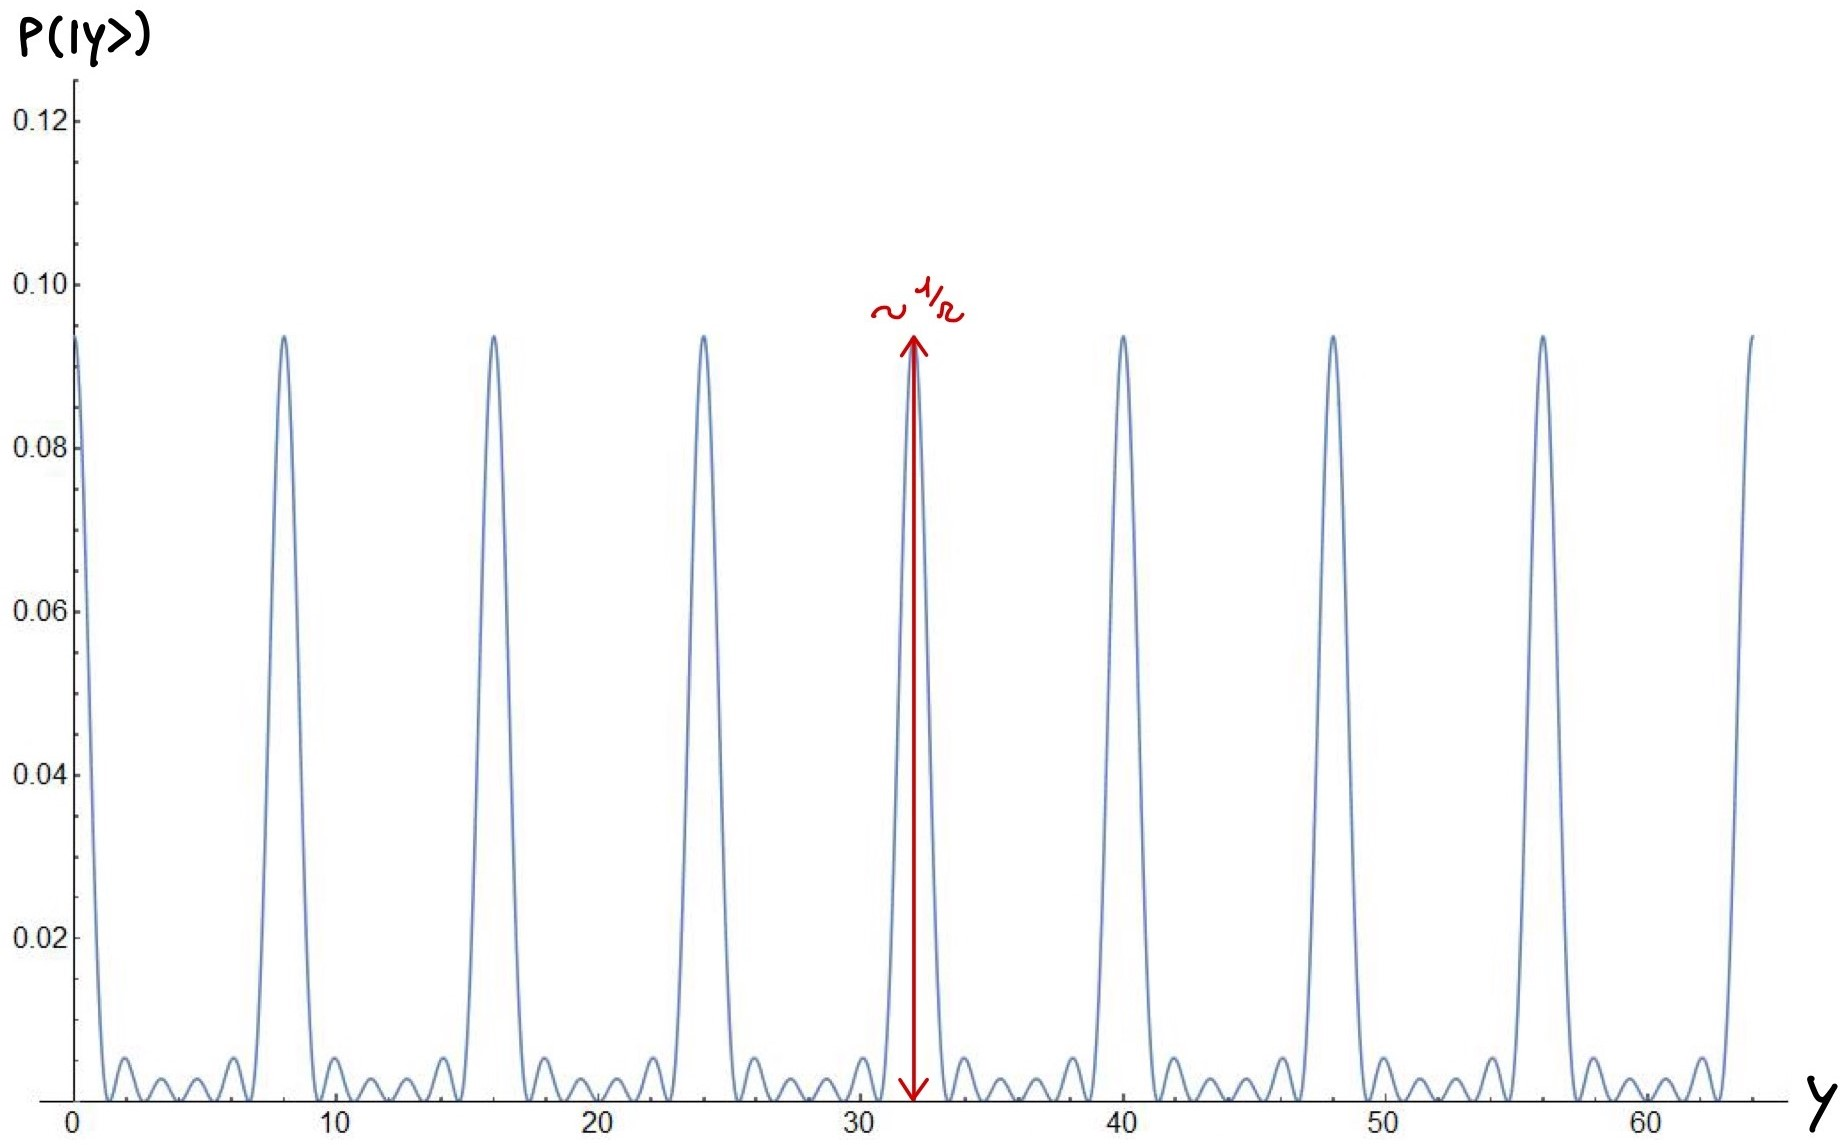
\includegraphics[scale=0.325]{images/probability_y}
    \caption{Esempio di grafico della probabilità di misurare $y$ della formula \eqref{probability_y}, dove $0 \leqslant y \leqslant 2^n$. In questo esempio si è usato $n = m = 6$ e $r = 8$. Si noti come il numero di picchi sia $\order{r}$ e la loro altezza, come ordine di grandezza, comparabile a $1/r$.}
    \label{fig:probability_y}
\end{figure}
Notiamo che vi sono differenti picchi di diverse ampiezze: ciò è dovuto al fatto che ci sono valori di $y$ dove abbiamo interferenza costruttiva, mentre in altri si ha interferenza distruttiva. Nel realizzare tale grafico, però, abbiamo assunto che $y \in \mathbb{R}$, ma bisogna ricordare che $y\in \mathbb{Z}$, quindi si tratta di un'approssimazione perché non tutti i punti della curva devono essere disegnati ! In realtà, per valori di $n$ molto grandi $2^n$ è enorme quindi la discretizzazione è minima e quasi impercettibile. I punti in cui la probabilità è maggiore, in corrispondenza dei picchi più alti, si ha $y = j\frac{2^n}{r}$ dove $j \in \mathbb{N}$. Per tali valori, gli esponenziali dentro la probabilità in \eqref{probability_y} non sono altro che $e^{2\pi i j k}=1$ perché $j, k \in \mathbb{Z}$, quindi la \eqref{probability_y} diventa:
\begin{equation*}
    P(\ket{y}) = \frac{1}{m 2^n} \abs{\sum_{k=0}^{m-1} 1}^2 = \frac{m^2}{m2^n} = \frac{m}{2^n} \, ,
\end{equation*}
il quale è il valore massimo della probabilità. Per capire per quale ragione abbiamo indicato nel grafico \ref{fig:probability_y} che l'altezza dei picchi è di circa $1/r$, ricordiamo che $2^n \sim N^2$, $r \sim N$ e anche $m \sim N$, per cui:
\begin{equation*}
    P(\ket{y}) = \frac{m}{2^n} \sim \frac N{N^2} \sim \frac 1 N \sim \frac 1 r \, .
\end{equation*}
Notiamo che sebbene abbiamo disegnato una funzione continua, l'approssimazione è comunque molto buona perché la probabilità totale è correttamente normalizzata a 1: infatti l'altezza dei picchi per il loro numero non è altro che $\frac{1}{r} \times m \sim \frac{1}{r} \times r \simeq 1$, quindi gran parte della probabilità è saturata i corrispondenza dei picchi (si può dimostrare che nel limite in cui $n \to \infty$ i picchi tendono a delle delta function). 

\noindent Un risultato fondamentale è che passando attraverso delle manipolazioni algebriche di seno e coseno, si può dimostrare che si ha circa il $40$\% di possibilità ($P(\ket{y}) = \frac{4}{\pi^2}$) di misurare $y$ e ottenere un valore che si trovi in prossimità di uno di questi picchi con un errore di circa $\frac 12$: ricordando che i picchi sono situati in $y = j \frac{2^n}{r}$, possiamo formalmente scrivere che
\begin{equation}
    \abs{y-j\frac{2^n}{r}} < \frac 12 \, , \quad \Rightarrow \quad 
    \abs{\frac y{2^n}-\frac jr} < \frac 1{2^{n+1}} \, ,
    \label{eq:shor2}
\end{equation}
dove abbiamo diviso per $2^n$. Stiamo quindi dicendo che una misura di $y$ soddisfa la disuguaglianza \eqref{eq:shor2} il 40\% delle volte. Possiamo estrarre $r$ dalla \eqref{eq:shor2} ? Innanzitutto notiamo che, essendo $0 \leqslant y \leqslant 2^n$, abbiamo $0 \leqslant \frac{y}{2^n} \leqslant 1$. Se $n = 2 n_0$ allora avremo $2^{n}=2^{2n_0}=N^2$, quindi quando la \eqref{eq:shor2} è verificata esiste un singolo numero razionale della forma $\frac j r$ che la  soddisfa e dal quale è possibile estrarre $r$. 

\noindent La logica è mostrata nel disegno della figura \ref{fig:inequality_40}: prendeno il segmento $[0,1]$ e suddividendolo in step uguali di lunghezza $\frac{1}{2^n}$, possiamo rappresentare con delle barrette verticali tutti i possibili valori di $y$ tali che $0 \leqslant \frac{y}{2^n} \leqslant 1$. La disuguaglianza \eqref{eq:shor2} ci dice che il numero $\frac{j}{r}$ (indicato con una "$\times$" azzurra) è vicino a $\frac{y}{2^n}$ con una distanza minore di $\frac{1}{2^{n+1}}$. 
\begin{figure}[!h]
    \centering
    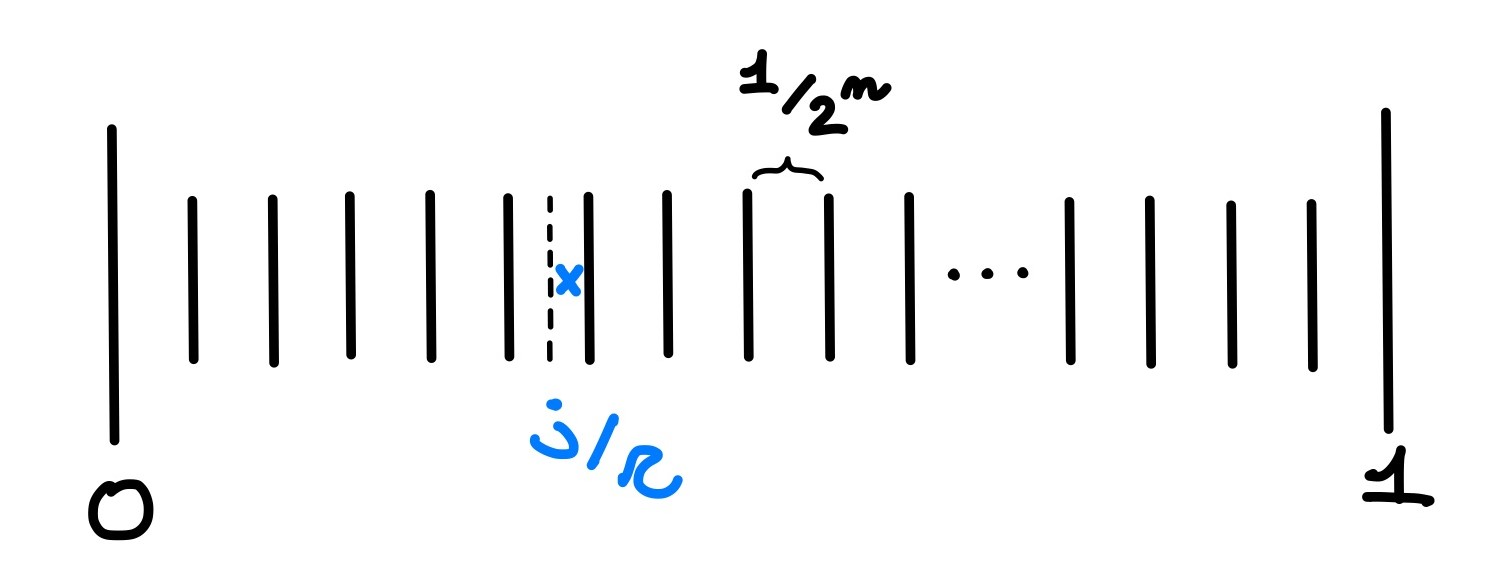
\includegraphics[scale=0.3]{images/inequality_40}
    \caption{Rappresentazione geometrica della disuguaglianza \eqref{eq:shor2}.}
    \label{fig:inequality_40}
\end{figure}

\noindent La domanda che possiamo porci è se esista più di un numero razionale che soddisfi questa particolare proprietà. Supponiamo per assurdo che esistano due numeri razionali $\frac{j_1}{r_1}$ e $\frac{j_2}{r_2}$ che soddisfano la disuguaglianza \eqref{eq:shor2} (e la condizione per cui $r_1, r_2 < N$). Allora la differenza tra questi due numeri è
\begin{equation}\label{difference_rational_numers}
    \frac{j_1}{r_1} - \frac{j_2}{r_2} = \frac{r_2j_1-r_1j_2}{r_1r_1} \, ,
\end{equation}
tuttavia il numeratore è un intero e il denominatore è di ordine $\order{N^2}$: essendo $r_1, r_2 < N$ allora il denominatore è strettamente minore di $N^2$ quindi la \eqref{difference_rational_numers} è $\geqslant \frac 1{N^2} = \frac{1}{2^n}$, che è proprio la larghezza degli step in cui abbiamo suddiviso $[0,1]$. Questo significa che se ci sono due soluzioni della \eqref{eq:shor2} allora la distanza tra le due deve necessariamente essere più grande della misura dello step: in un dato step è possibile trovare una sola soluzione, ossia un solo numero razionale che verifica la \eqref{eq:shor2}.

\noindent Riassumendo: misurando un valore $y$ che soddisfa la \eqref{eq:shor2} otteniamo un unico numero razionale $\frac{j}{r}$. Il punto chiave è quindi trovare  $\frac jr$, tuttavia questo non è così semplice, perché quello che si ottiene dalla misura è un numero scritto in forma decimale, il quale vorremmo poterlo scrivere come rapporto tra razionali. Nonostante ciò facciamo uso del seguente risultato di teoria dei numeri che non dimostreremo. Riscriviamo la disuguaglianza \eqref{eq:shor2} come
\begin{equation*}
    \abs{x-\frac jr} \leqslant \frac 1{2r^2} \, , \; \text{ dove } x\in[0,1] \, .
\end{equation*}
Il valore $x$ è dato dalla misura mentre lo scopo è quello di trovare un numero razionale $\frac jr$ che soddisfi questa disuguaglianza. Il risultato dalla teoria dei numeri asserisce che questo valore appare nell'espansione in frazione continua del numero $x$:
\begin{equation*}
    x=\frac{1}{x_0+\frac{1}{x_1+\frac{1}{x_2+\ldots}}} \, .
\end{equation*}

\begin{esempio}[Espansione in frazione continua]
    Supponiamo di considerare il numero $x=0.256789$. Prendendone l'inverso avremo $\frac{1}{x} = \frac{1}{0.256789} = 3.8942478 \ldots$. Da questo risultato è evidente che $x_0 = 3$. Nello step successivo si calcola $x_1$: calcoliamo $\frac{1}{x}-3$ e poi $\left( \frac{1}{x}-3 \right)^{-1}$, la cui parte intera è $x_1$. Iterando all'infinito questo procedimento si ottiene l'espansione in frazione continua di $x$:
    \begin{equation*}
        x=\frac{1}{3+\frac{1}{1+\frac{1}{8+\dots}}} \, .
    \end{equation*}
    Ad ogni step si ottiene quindi un'approssimazione razionale di $x$, infatti il set di numeri razionali che approssimano il suo valore è dato da $\left\{ \frac 13, \frac 14, \frac 9{35}, \frac {19}{74}, \frac{104}{405}, \dots \right\}$. Più si procede, meglio approssimato sarà il valore di $x$. Il teorema ci dice che a un certo punto possiamo trovare il valore di $\frac jr$ all'interno di questo insieme e questo con una probabilità del 100\%. 
\end{esempio}

\noindent Tuttavia di questo procedimento vanno fatte delle opportune precisazioni:
\begin{itemize}
    \item Supponiamo che $j$ e $r$ abbiano dei fattori comuni (e questo ovviamente non lo sapremo mai), allora il valore di $r$ può essere diverso, infatti:
    \begin{equation*}
        \frac jr=\frac{j_0k}{r_0k}=\frac{j_0}{r_0} \, ,
    \end{equation*}
    quindi mediante la procedura sopraelencata, al posto di trovare il periodo cercato, si ottiene $r_0$. Nonostante ciò si è trovato un divisore di $r$, quindi prendendo la forma analitica di $f$ si può provare a calcolare $f(x+r_0)$, $f(x + 2 r_0)$, $f(x + 3 r_0)$, \dots fino a quando effettivamente si trova un valore uguale a  $f(x)$.
    
    \item Talvolta si possono misurare dei valori $y$ che non soddisfano la disuguaglianza \eqref{eq:shor2} (la probabilità di soddisfarla è infatti del 40\%). In tal caso basta semplicemente ricominciare l'algoritmo da capo con una nuova esecuzione del circuito e della QFT fino a quando non si ottiene un valore di $y$ che soddisfi la \eqref{eq:shor2}. Inoltre è possibile dimostrare che la probabilità che la \eqref{eq:shor2} sia soddisfatta cresce fino al 90\% se si sa a priori che $r < \frac N2$.
\end{itemize}
Concludiamo la discussione dicendo che lo stesso tipo di algoritmo può essere utilizzato per calcolare i \textit{logaritmi discreti}, oppure per la simulazione di sistemi quantistici (si possono calcolare gli autovalori di matrici unitarie molto grandi che servono per il calcolo degli autovalori delle relative hamiltoniane e degli evoluti temporali).
    %%%%%%%%%%%%%
% LECTURE 9 %
%%%%%%%%%%%%%
\chapter{Sistemi aperti}

\lecture{9}{05/11/2021}
\section{Matrice densità}
Il formalismo della \textbf{matrice densità} viene solitamente introdotto per affrontare situazioni in cui sono presenti sia un'incertezza quantistica, intrinseca alla QM, che un'incertezza classica, dovuta all'ignoranza su alcune configurazioni del sistema. Spesso viene introdotta nell'ambito della fisica statistica, tuttavia viene largamente utilizzata anche in altri contesti. 

\noindent Ad esempio: supponiamo di considerare un laboratorio e un ambiente esterno in cui è immerso; spesso, per descrivere la fisica del sistema completo, non si possono tenere in considerazione tutti i gradi di libertà dell'ambiente, così si assume che esista un'opportuna descrizione del laboratorio (nel quale potrebbe esserci un qubit o un apparato sperimentale) più l'ambiente e si prende una traccia (capiremo tra un attimo cosa significhi) su tutti i gradi di libertà dell'ambiente. In questo modo si ottiene una \textbf{descrizione efficace} del laboratorio, la quale contiene "nascosta" la nostra ignoranza relativa all'ambiente. 

\noindent Vediamo la definizione generale:

\begin{definizione}[\textbf{Matrice Densità}]
    Siano $\ket{\psi_i}$ un insieme di stati quantistici con probabilità classica $p_i$ ($\sum_i p_i = 1$), ossia la probabilità di realizzare ogni stato $\ket{\psi_i}$ è data da $p_i$. Indichiamo con $\{ p_i, \ket{\psi_i} \}$ l'insieme di tali stati con le rispettive probabilità (assumiamo che $\braket{\psi_i} = 1$). Si definisce \textbf{matrice densità} (o \textbf{operatore densità}) $\rho$ la seguente
    \begin{equation}\label{density_matrix}
        \rho = \sum_i p_i \ket{\psi_i} \otimes \bra{\psi_i} \, .
    \end{equation}
\end{definizione}

\noindent Si noti che, come evidenziato, le $p_i$ sono probabilità \textit{classiche} poiché è già intrinseca ad ogni stato $\ket{\psi_i}$ la descrizione mediante probabilità \textit{quantistica}. Chiaramente $\rho$, in quanto prodotto esterno, agisce come un operatore sugli stati dello spazio di Hilbert. È importante sottolineare che che gli stati $\ket{\psi_i}$ sono normalizzati ma non necessariamente ortogonali. 

\noindent L'introduzione della \eqref{density_matrix} è utile perché permette di scrivere differenti quantità in forma compatta. Ad esempio, la media di un'osservabile $A$ può essere scritta come
\begin{equation}\label{expval_A_rho}
    \expval{A} = \Tr (\rho A) \, .
\end{equation}
\begin{proof}
    Scriviamo 
    \begin{equation*}
        \Tr (\rho A) = \sum_i p_i \Tr \left( \ketbra{\psi_i} A \right) = \sum_i p_i \expval{A}{\psi_i} = \expval{A} \, ,
    \end{equation*}
    dove nel secondo passaggio abbiamo utilizzato la proprietà ciclica della traccia per muovere il ket a destra. Notiamo che questa operazione può essere svolta per la ragione seguente: in generale per gli operatori si ha $\Tr B = \sum_n \expval{B}{n}$ dove $\{ \ket{n} \}$ è una base ortonormale, perciò nel passaggio sopra possiamo scrivere
    \begin{equation*}
        \Tr \left( \ketbra{\psi_i} A \right) = \sum_n \braket{n}{\psi_i} \mel{\psi_i}{A}{n} = \sum_n \mel{\psi_i}{A}{n} \braket{n}{\psi_i} = \expval{A}{\psi_i} \, ,
    \end{equation*}
    dove nell'ultimo passaggio abbiamo utilizzato la relazione di completezza $\mathbb{I} = \sum_n \ketbra{n}$.
\end{proof}

\noindent Se si possiede solamente uno stato $\ket{\psi}$, esso viene chiamato \textbf{stato puro}, quindi la matrice densità si scriverà come $\rho = \ketbra{\psi}$. Al contrario, un insieme di stati $\{ p_i, \ket{\psi_i} \}$, con almeno 2 probabilità $p_i \neq 0$, avrà matrice densità $\rho = \sum_i p_i \ketbra{\psi_i}$ ed è chiamato \textbf{stato misto} o \textbf{miscela di stati} (nota anche come \textbf{mixture}). Ribadiamo nuovamente che in quest'ultima situazione l'incertezza classica $p_i$ si va ad aggiungere all'incertezza puramente quantomeccanica degli stati quantistici.

\begin{esempio}[\textbf{Miscela in Meccanica Statistica}]
    Il più semplice esempio di miscela di stati in meccanica statistica è costituito dall'insieme di stati $\{ E_n, \ket{n} \}$, dove $H \ket{n} = E_n \ket{n}$, in cui assegniamo ad ogni stato una probabilità classica 
    \begin{equation*}
        P(E_n) = \frac{e^{-\frac{E_n}{k_BT}}}{Z} \, , \; \text{ con } \; Z = \sum_n e^{-\frac{E_n}{k_BT}} \, ,
    \end{equation*}
    dove $Z$ è chiamata \textbf{funzione di partizione}. Quindi per studiare un tale sistema dal punto di vista quantistico possiamo dire che in aggiunta all'incertezza quantistica ci sono altre probabilità classiche $P(E_n)$ dipendenti dalla temperatura. Per un tale sistema la matrice densità non è altro che
    \begin{equation*}
        \rho = \sum_n p_n \ketbra{n} \, , \; \text{ dove } \; p_n \equiv P(E_n) = \frac{e^{-\frac{E_n}{k_BT}}}{Z} \, . 
    \end{equation*}
\end{esempio}

\noindent Vediamo immediatamente l'esempio dei qubit per capire la differenza della matrice densità nel caso di uno stato puro e per miscele di stati:

\begin{esempio}[\textbf{Singolo qubit: stato puro}]
    Immaginiamo un qubit nello stato $\ket{0}$. La matrice \eqref{density_matrix} non è altro che
    \begin{equation*}
        \rho = \ketbra{0} = 
        \begin{pmatrix}
            1 \\ 0
        \end{pmatrix} \otimes 
        \begin{pmatrix}
            1 & 0
        \end{pmatrix} 
        = 
        \begin{pmatrix}
            1 & 0 \\ 0 & 0
        \end{pmatrix} \, ,
    \end{equation*}
    dove nell'ultimo passaggio abbiamo utilizzato il prodotto di Kronecker della definizione \ref{def:Kronecker}.
\end{esempio}

\begin{esempio}[\textbf{Singolo qubit: miscela di stati}]\label{example:mixture_qubit}
    Si consideri un qubit nella miscela di stati in cui $\ket{0}$ è dato con probabilità $p$ e $\ket{1}$ con probabilità $1-p$ (non stiamo prendendo la solita sovrapposizione di stati della QM). Allora la matrice densità risulterà
    \begin{equation*}
        \rho = p \ketbra{0} + (1-p) \ketbra{1} = p 
        \begin{pmatrix}
            1 & 0 \\ 0 & 0
        \end{pmatrix} + 
        (1-p)
        \begin{pmatrix}
            0 & 0 \\ 0 & 1
        \end{pmatrix}
        =
        \begin{pmatrix}
            p & 0 \\ 0 & 1-p
        \end{pmatrix} \, .
    \end{equation*} 
\end{esempio}

\noindent Notiamo che dal punto di vista dell'informazione, nello stato puro la matrice densità ha solamente un'entrata: non vi è alcuna incertezza classica (solamente quantistica). Al contrario, per la miscela di stati abbiamo il caso della maggior incertezza possibile quando $p = \frac{1}{2}$ perché $\rho = \frac{1}{2} \mathbb{I}$. In generale, per matrici diagonali,  sono miscele le configurazioni in cui pi\`u di un'entrata diagonale \`e non nulla. Si noti dall'esempio \ref{example:mixture_qubit} che sulle entrate diagonali di $\rho$ si può leggere l'incertezza classica collegata agli stati $\ket{0}$ e $\ket{1}$. 

\noindent Questi esempi erano molto semplici perché $\rho$ è diagonale: la matrice densità non è in generale diagonale né per gli stati puri né per le miscele. Vediamo alcuni esempi:

\begin{esempio}[\textbf{Stato puro: $\rho$ non diagonale}]\label{example:rho_non_diagonal_pure}
    Consideriamo il caso dello stato puro di un qubit nella sua forma più generale, ossia $\ket{\psi} = \alpha \ket{0} + \beta \ket{1}$. La \eqref{density_matrix} diventa una matrice non diagonale, infatti
    \begin{equation*}
        \rho = \ketbra{\psi} = 
        \begin{pmatrix}
            \alpha \\ \beta
        \end{pmatrix}
        \otimes
        \begin{pmatrix}
            \alpha^\ast & \beta^\ast
        \end{pmatrix} 
        = 
        \begin{pmatrix}
            \abs{\alpha}^2 & \alpha \beta^\ast \\ \alpha^\ast \beta & \abs{\beta}^2
        \end{pmatrix} \, .
    \end{equation*}
\end{esempio}

\noindent Si noti dall'esempio precedente la differenza tra le entrate diagonali e non: su quelle diagonali vi sono le probabilità quantistiche del risultato di una misura, mentre su quelle non diagonali sono presenti dei prodotti tra $\alpha$ e $\beta$ che misurano, in un certo senso, l'interferenza (sovrapposizione) tra $\ket{0}$ e $\ket{1}$.

\begin{esempio}[\textbf{Miscela: $\rho$ non diagonale}]\label{example:rho_non_diagonal_mixture}
    Supponiamo di avere la miscela costituita dal 50\% di probabilità di avere $\ket{0}$ e dal $50\%$ di probabilità di avere $\ket{+} = \frac{1}{\sqrt{2}} (\ket{0} + \ket{1})$. In questo caso $\rho$ non è diagonale ed è data da una combinazione lineare di stati non ortogonali:
    \begin{equation*}
        \rho = \frac{1}{2} \ketbra{0} + \frac{1}{2} \ketbra{+} = \frac{1}{2} \begin{pmatrix} 1 & 0 \\ 0 & 0 \end{pmatrix} + \frac{1}{4} \begin{pmatrix} 1 \\ 1 \end{pmatrix} \otimes \begin{pmatrix} 1 & 1 \end{pmatrix} = \begin{pmatrix} \frac{3}{4} & \frac{1}{4} \\ \frac{1}{4} & \frac{1}{4} \end{pmatrix} \, . 
    \end{equation*}
\end{esempio}

\noindent Vediamo alcune proprietà generali della matrice densità:
\begin{enumerate}
    \item \textit{$\rho$ è hermitiana e positiva}. 
    \begin{proof}
        Ricordando che $p_i \geq 0 \in \mathbb{R}$ allora
        \begin{equation*}
            \left( \sum_i p_i \ketbra{\psi_i} \right)^\dag = \sum_i p_i \ketbra{\psi_i} \, .
        \end{equation*}
        La positività di un operatore $A$ è data dalla proprietà $\expval{A}{\phi} \geq 0$ per ogni $\ket{\phi}$, quindi
        \begin{equation*}
            \expval{\rho}{\phi} = \bra{\phi} \sum_i p_i \ket{\psi_i} \braket{\psi_i}{\phi} = \sum_i p_i \braket{\phi}{\psi_i} \underbrace{\braket{\psi_i}{\phi}}_{\braket{\phi}{\psi_i}^\ast} = \sum_i p_i \abs{\braket{\phi}{\psi_i}}^2 \geq 0 \, .
        \end{equation*}
    \end{proof}
    
    \item $\Tr \rho = 1$.
    \begin{proof}
        \begin{equation*}
            \Tr \left[ \sum_i p_i \ketbra{\psi_i} \right] = \sum_i p_i \Tr \ketbra{\psi_i} = \sum_i p_i \braket{\psi_i} = 1 \, ,
        \end{equation*}
        dove nel penultimo passaggio abbiamo usato la proprietà ciclica della traccia come nella dimostrazione della \eqref{expval_A_rho}.
    \end{proof}
    
    \item \textit{$\Tr \rho^2 \leq 1$ e $\Tr \rho^2 = 1$ solo per gli stati puri}.
    \begin{proof}
        Dato che $\rho$ è hermitiana allora può essere diagonalizzata, quindi $\rho \ket{n} = \rho_n \ket{n}$. In particolare avremo
        \begin{equation}\label{diagonalization_rho}
            \rho = \sum_i p_i \ketbra{\psi_i} \equiv \sum_n \rho_n \ketbra{n} \, ;
        \end{equation}
        quindi la matrice densità è scrivibile come somma del prodotto tra i proiettori nella direzione degli autospazi e dei corrispondenti autovalori. Notiamo che la formula precedente consiste di fatto nella diagonalizzazione in notazione di Dirac. Chiaramente in generale $p_i \neq \rho_i$! Dato che $\Tr \rho = 1$ allora dalla precedente si ha che $\sum_n \rho_n = 1$. Cerchiamo di valutare $\Tr \rho^2 = \sum_n \rho_n^2$: dato che la matrice densità è hermitiana e positiva allora $\rho_n \geq 0 \in \mathbb{R}$, ma al tempo stesso si deve avere $0 \leq \rho_n \leq 1$ poiché $\sum_n \rho_n = 1$. Ma allora
        \begin{equation*}
            0 \leq \rho_n^2 \leq \rho_n \leq 1 \, , \quad \Rightarrow \quad \sum_n \rho_n^2 \leq \sum_n \rho_n = 1 \, .
        \end{equation*}
        Il caso limite è dato da
        \begin{equation*}
            \sum_n \rho_n^2 = 1 = \sum_n \rho_n \quad \Leftrightarrow \quad \rho_n = \rho_n^2 \, , \; \forall n \, ,
        \end{equation*}
        ma per numeri tra 0 e 1 questo è vero solamente per $\rho_n = 1 \lor \rho_n = 0$: solamente un valore è diverso da 0 (uguale a 1) mentre tutti gli altri sono 0, quindi $\rho = \ketbra{n}$ per un particolare $n$, ossia si tratta di uno stato puro. 
    \end{proof}
    Si noti che la formula $\left[ \Tr \rho^2 = 1 \Leftrightarrow \text{ stato puro} \right]$ è un criterio per stabilire se effettivamente uno stato è puro. Inoltre, essendo $\rho$ hermitiana, può sempre essere diagonalizzata secondo la \eqref{diagonalization_rho} e quindi la sua forma non è unica (si pensi ai casi degli esempi \ref{example:rho_non_diagonal_pure} e \ref{example:rho_non_diagonal_mixture} che possono essere diagonalizzati).
\end{enumerate}

\noindent Torniamo al caso dei qubit. Avevamo visto che la più generale matrice hermitiana $2 \times 2$ può essere scritta come $\rho = a_0 \mathbb{I} + \vec{a} \cdot \vec{\sigma}$ con $a_0, \vec{a} \in \mathbb{R}$, ma $\Tr \rho = 1$ e quindi, dato che le matrici di Pauli hanno traccia nulla, avremo $1 = 2 a_0$, ossia $a_0 = \frac{1}{2}$. Possiamo allora scrivere la matrice densità come
\begin{equation}\label{density_matrix_Pauli}
    \rho = \frac{\mathbb{I} + \vec{r} \cdot \vec{\sigma}}{2} \, , \; \text{ dove } \; r_i \in \mathbb{R} \, .
\end{equation}
Quali sono gli autovalori di $\rho$? Sappiamo che $\vec{r} \cdot \vec{\sigma}$ è lo spin in direzione $\vec{r}$, il quale ha autovalori $\abs{\vec{r}\,}$ e $-\abs{\vec{r}\,}$, inoltre $\rho$ è hermitiana, quindi
\begin{equation*}
    \eig(\rho) \equiv \lambda = \frac{1 \pm \abs{\vec{r} \,}}{2} \geq 0 \, , \quad \Rightarrow \quad \abs{\vec{r}\,} \leq 1 \, . 
\end{equation*}
Calcoliamo ora $\Tr \rho^2$ sempre usando la \eqref{density_matrix_Pauli}:
\begin{equation*}
    \Tr \rho^2 = \Tr \left[ \frac{1}{4} \left( \mathbb{I} + 2 \vec{r} \cdot \vec{\sigma} + \abs{\vec{r}\,}^2 \right) \right] = \frac{1 + \abs{\vec{r}\,}^2}{2} \leq 1 \, ,
\end{equation*}
dove abbiamo usato il risultato seguente
\begin{equation*}
    r_i r_j \sigma_i \sigma_j = r_i r_j \left( \delta_{ij} \mathbb{I} + i \varepsilon_{ijk} \sigma_k \right) = \abs{\vec{r}\,}^2 + i (\varepsilon_{kij} r_i r_j) \sigma_k = \abs{\vec{r}\,}^2 + i \underbrace{(\vec{r} \times \vec{r}\,)}_0 \cdot \, \vec{\sigma} = \abs{\vec{r}\,}^2 \, .
\end{equation*}
Notiamo che per gli stati puri $\frac{1+ \abs{\vec{r}\,}^2}{2} = 1 \Leftrightarrow \abs{\vec{r}\,}^2 = 1$, quindi possiamo impiegare nuovamente la descrizione grafica con la sfera di Bloch che abbiamo introdotto nella Sottosezione \ref{subsec:Bloch}. Associamo il punto dato da $\vec{r}$ con la matrice densità \eqref{density_matrix_Pauli} in maniera tale da estendere questa descrizione anche ai punti interni della sfera (si veda la Figura \ref{fig:BlochSphere} a Pagina \pageref{fig:BlochSphere}): i punti sulla superficie sono stati puri, mentre quelli all'interno sono delle miscele di stati. Tenendo presente la Figura \ref{fig:BlochSphere2} a Pagina \pageref{fig:BlochSphere2}, focalizziamo la nostra attenzione su due direzioni precise:
\begin{itemize}
    \item Consideriamo l'asse $z$: in tal caso avremo $\vec{r} = (0, 0, r)$ con $r \in [-1, 1]$. Chiaramente i due stati corrispondenti ai punti sulla superficie sono $\ket{0}$ per $z=1$ e $\ket{1}$ per $z = -1$. La matrice densità non è altro che
    \begin{equation}\label{rho_z_Bloch}
        \rho = \frac{\mathbb{I}}{2} + \frac{r}{2} \sigma_3 = 
        \begin{pmatrix}
            \frac{1+r}{2} & 0 \\ 0 & \frac{1-r}{2}
        \end{pmatrix}
        \equiv
        \begin{pmatrix}
            p & 0 \\ 0 & 1-p
        \end{pmatrix} \, , \; \text{ con } \; p = \frac{1+r}{2} \, ;
    \end{equation}
    si tratta della stessa forma dell'Esempio \ref{example:mixture_qubit}: si ha una miscela di stati con probabilità classiche $p$ di avere $\ket{0}$ e $1-p$ di avere $\ket{1}$. 
    
    \item Consideriamo ora, invece, l'asse $x$: in tal caso $\vec{r} = (r, 0, 0)$ e gli stati sulla superficie (intersezione sfera con asse $x$) sono $\ket{+}$ per $x = 1$ e $\ket{-}$ per $x = -1$. La \eqref{density_matrix_Pauli} non è altro che
    \begin{equation}\label{rho_x_Bloch}
        \rho = \frac{\mathbb{I}}{2} + \frac{r}{2} \sigma_1 =
        \begin{pmatrix}
            \frac{1}{2} & \frac{r}{2} \\ \frac{r}{2} & \frac{1}{2}
        \end{pmatrix} \, ;
    \end{equation}
    perciò i punti corrispondenti a $\ket{+}$ e $\ket{-}$ sono gli stati puri nella direzione in cui si sta misurando lo spin, mentre tutti gli altri punti intermedi lungo $x$ sono una miscela di $\ket{+}$ e $\ket{-}$. 
\end{itemize}

\noindent Notiamo che il punto $\vec{r} = 0$ è l'unico punto comune a tutti e 3 gli intervalli nelle 3 direzioni spaziali: esso corrisponde alla massima indeterminazione possibile, infatti
\begin{equation*}
    \rho = \frac{\mathbb{I}}{2} = 
    \begin{pmatrix}
        \frac{1}{2} & 0 \\ 0 & \frac{1}{2}
    \end{pmatrix} \, ,
\end{equation*}
il quale non è altro che una sovrapposizione dei due autostati corrispondenti ognuno una probabilità classica del 50\%. Un fatto importante da sottolineare è che la matrice precedente può essere ottenuta sia dalla \eqref{rho_z_Bloch} che dalla \eqref{rho_x_Bloch} ponendo $p = \frac{1}{2}$ e $r = 0$: solamente conoscendo la matrice densità di un sistema non siamo in grado di distinguere la miscela di stati in cui ci troviamo!

\section{Sottosistemi e traccia parziale}
Torniamo ad affrontare alcuni casi interessanti dal punto di vista della fisica dei qubit. Il formalismo della matrice densità risulta utile quando si hanno sistemi bipartiti tali che $\mathcal{H} = \mathcal{H}_A \otimes \mathcal{H}_B$. Supponiamo che Alice si trovi in un laboratorio descritto da $\mathcal{H}_A$ e che Bob invece sia in un altro laboratorio descritto da $\mathcal{H}_B$: la matrice densità è utile quando si vuole studiare la fisica dal punto di vista di Alice, la quale ignora il laboratorio di Bob; Alice vorrebbe ignorare parte dello spazio di Hilbert totale perché non ne ha l'accesso completo.  Questo fatto, vedremo, porta ad una descrizione fisica in termini di miscele di stati anche se si era partiti da uno stato puro in $\mathcal{H}$. 

\noindent Che cosa significa fare esperimenti dal punto di vista di Alice? Significa che Alice effettua misure di osservabili della forma $O = O_A \otimes \mathbb{I}_B$, quindi agisce solamente nel proprio laboratorio senza fare nulla sul laboratorio di Bob. Immaginiamo che i due laboratori siano soggetti a dell'indeterminazione classica, quindi il sistema totale è ben descritto da un'opportuna matrice densità $\rho$. Siamo interessati al sottosistema descritto da $\mathcal{H}_A$: chiamiamo $\{ \ket{nm} \}$ la base dello spazio di Hilbert totale $\mathcal{H}$ dove $\ket{nm} \equiv \ket{n}_A \otimes \ket{m}_B$ con $\ket{n}_A \in \mathcal{H}_A$ e $\ket{m}_B \in \mathcal{H}_B$. Calcoliamo il valor medio di $O$ mediante la \eqref{expval_A_rho}:
\begin{align*}
    \expval{O} &= \Tr (O \rho) = \sum_{n,m} \expval{O \rho}{nm} \\
    &= \sum_{\substack{n,m \\ n', m'}} \mel{nm}{O_A \otimes \mathbb{I}_B}{n'm'} \mel{n'm'}{\rho}{nm} \\
    &= \sum_{\substack{n,m \\ n', m'}} \mel{n}{O_A}{n'} \underbrace{\braket{m}{m'}}_{\delta_{mm'}} \mel{n'm'}{\rho}{nm} \\
    &= \sum_{n,m,n'} \mel{n}{O_A}{n'} \mel{n'm}{\rho}{nm} \\
    &= \sum_{n,n'} \mel{n}{O_A}{n'} \sum_m \mel{n'm}{\rho}{nm} \, ,
\end{align*}
dove nella seconda riga abbiamo inserito una relazione di completezza nello spazio $\mathcal{H}$: $\mathbb{I} = \sum_{n',m'} \ketbra{n'm'}$. Definiamo ora il seguente oggetto
\begin{equation}\label{rho_A}
    \mel{n'}{\rho_A}{n} \equiv \sum_m \mel{n'm}{\rho}{nm} \, ,
\end{equation}
dove chiaramente $\rho_A$ agisce solamente su $\mathcal{H}_A$. In questo modo la precedente diventa
\begin{equation*}
    \expval{O} = \sum_{n,n'} \mel{n}{O_A}{n'} \mel{n'}{\rho_A}{n} = \sum_n \expval{O_A \rho_A}{n} = \Tr (O_A \rho_A) \, ,
\end{equation*}
dove abbiamo tolto, nel penultimo passaggio, una relazione di completezza in $\mathcal{H}_A$. In definitiva abbiamo ricavato
\begin{equation}\label{expval_O_partial_trace}
    \expval{O} = \Tr (O_A \rho_A) \, .
\end{equation}
Siamo partiti dal considerare un valor medio di una grandezza di tutto lo spazio di Hilbert, ma abbiamo ricavato una formula che considera solamente oggetti che agiscono su $\mathcal{H}_A$! La relazione \eqref{expval_O_partial_trace} permette di dare una \textbf{descrizione efficace} di tutti i gradi di libertà del sistema prendendo una cosiddetta "\textbf{traccia parziale sullo spazio di Hilbert $\mathcal{H}_B$}". 

\noindent Omettendo $n,n'$ ad entrambi i membri, possiamo scrivere la definizione \eqref{rho_A} in forma più compatta come
\begin{equation*}
    \rho_A = \sum_m \expval{\rho}{m} \equiv \Tr_B \rho \, ;
\end{equation*}
risulta ancora più evidente che $\rho_A$ sia costruita prendendo una traccia sui gradi di libertà del laboratorio di Bob, tuttavia notiamo che quest'ultima formula è un po' fuorviante dato che $\rho_A$ è un operatore e il RHS sembrerebbe invece un numero: il simbolo "$\Tr_B$" non produce un numero, bensì un operatore agente unicamente su $\mathcal{H}_A$.

\noindent Vediamo immediatamente due semplici esempi per fissare meglio questi concetti. 
\begin{esempio}[\textbf{Fisica "fattorizzata"}]
    Supponiamo che la fisica di un sistema possa essere "fattorizzata" scrivendo $\rho = \rho_A \otimes \rho_B$. Supponiamo di voler studiare il sistema dal punto di vista di Alice:
    \begin{equation*}
        \Tr_B \rho = \Tr_B (\rho_A \otimes \rho_B) = \sum_m \expval{\rho_A \otimes \rho_B}{m} = \rho_A \otimes \sum_m \expval{\rho_B}{m} = \rho_A \underbrace{\Tr \rho_B}_1 = \rho_A \, ;
    \end{equation*}
    quindi se si vuole studiare la fisica di $\mathcal{H}_A$ e la fisica totale è disaccoppiata, ci si aspetta che prendere una traccia sui gradi di libertà esterni produca $\rho_A$: per effettuare una misura nel laboratorio di Alice bisogna solamente utilizzare $\rho_A$. 
\end{esempio}

\begin{esempio}[\textbf{Qubit in stati separabili}]
    Supponiamo che Alice e Bob condividano due qubit in uno stato separabile, $\ket{00}$ ad esempio, dove la prima entrata appartiene ad Alice e la seconda a Bob. Anche in una situazione come questa la fisica è fattorizzata e le misurazioni sono indipendenti perché il collasso dello stato non produce alcunché di nuovo. Cosa succede a $\rho$ dal punto di vista di Alice? Sappiamo che $\rho = \ketbra{00}$ quindi
    \begin{equation*}
        \rho_A \equiv \Tr_B \rho = \Tr_B \ketbra{00} = \sum_m \braket{m}{00} \braket{00}{m} = \ketbra{0} \, ,
    \end{equation*}
    dove nell'ultimo passaggio sopravvivono solamente i prodotti scalari per $m=0$. In questa situazione abbiamo ottenuto che $\rho_A$ corrisponde alla matrice densità di uno stato puro, perché metà delle paia di qubit appartengono ad Alice. 
\end{esempio}

\noindent Chiaramente, in analogia con gli stati separabili, i casi degli esempi precedenti non sono molto utili e interessanti. Vediamo, invece, che per stati entangled l'effetto della traccia diventa del tutto non banale:

\begin{esempio}[\textbf{Qubit in stati entangled}]
    Supponiamo che Alice e Bob condividano lo stato entangled $\ket{\psi} = \frac{1}{\sqrt{2}} \left( \ket{00} + \ket{11} \right)$ (come nell'esempio precedente ad Alice appartiene la prima entrata mentre a Bob la seconda). Scriviamo la matrice densità totale:
    \begin{equation*}
        \rho = \ketbra{\psi} = \frac{1}{2} \left( \ketbra{00} + \ketbra{00}{11} + \ketbra{11}{00} + \ketbra{11} \right) \, ;
    \end{equation*}
    si noti che lo stato $\ket{\psi}$ è puro nello spazio di Hilbert totale. Vediamo la matrice densità di Alice:
    \begin{equation*}
        \rho_A = \Tr_B \rho = \sum_m \expval{\rho}{m} = \expval{\rho}{0} + \expval{\rho}{1} \, ;
    \end{equation*}
    calcoliamo separatamente i due termini:
    \begin{align*}
        \expval{\rho}{0} &= \frac{1}{2} \left( \braket{0}{00} \braket{00}{0} + \braket{0}{00} \braket{11}{0} + \braket{0}{11} \braket{00}{0} + \braket{0}{11} \braket{11}{0} \right) = \frac{1}{2} \ketbra{0} \, , \\
        \expval{\rho}{1} &= \frac{1}{2} \left( \braket{1}{00} \braket{00}{1} + \braket{1}{00} \braket{11}{1} + \braket{1}{11} \braket{00}{1} + \braket{1}{11} \braket{11}{1} \right) = \frac{1}{2} \ketbra{1} \, ,
    \end{align*}
    quindi avremo semplicemente che
    \begin{equation*}
        \rho_A = \frac{1}{2} \left( \ketbra{0} + \ketbra{1} \right) = \frac{1}{2} \sum_n \ketbra{n} = \frac{\mathbb{I}}{2} \, .
    \end{equation*}
    Come sottolineato in precedenza, si tratta del caso peggiore possibile in cui tutto è completamente indeterminato: dal punto di vista di Alice c'è una totale casualità. 
\end{esempio}

\noindent Perciò anche se si parte da uno stato puro nello spazio di Hilbert totale (universo) e si decide di effettuare un esperimento solo localmente, la traccia parziale pu\`o trasformarlo  in una matrice densità: tracce parziali producono tipicamente matrici densità. 

\noindent Come ultima curiosità enunciamo il teorema seguente:
\begin{teorema}[\textbf{Teorema di purificazione}]
    Data la traccia parziale $\rho_A$ agente su $\mathcal{H}_A$, esiste sempre uno spazio di Hilbert più grande $\mathcal{H} = \mathcal{H}_A \otimes \mathcal{H}_B$ e uno stato puro $\ket{\psi} \in \mathcal{H}$ tale che
    \begin{equation*}
        \rho_A = \Tr_B \rho \, , \; \text{ con } \; \rho = \ketbra{\psi} \, .
    \end{equation*}
\end{teorema}
\end{document}
